%%&xelatex
\documentclass{sysuthesis}

\usepackage{layout}
\usepackage{indentfirst}% not needed if xecjk
\setlength{\parindent}{2em}
\usepackage{ifthen}
\usepackage{dcolumn}	% 
\usepackage{multirow}	%
\usepackage{mdwlist}	% 
\usepackage{verbatim}	% 
%\usepackage{subscript}	% \textsubscript without math
%\usepackage[superscript,nocompress,nobreak,nomove]{cite} % for overcite
\usepackage{amsmath}
\DeclareMathOperator{\diff}{d\!}
\DeclareMathOperator{\ee}{e}
\DeclareMathOperator{\imag}{i}
\usepackage{amsfonts}
\usepackage{amssymb}	% conflict with xunicode, thus go before it

\usepackage{ifxetex}
\ifxetex
\usepackage{xltxtra}
\usepackage{xunicode}
\usepackage{fontspec}	%[no-math]
\defaultfontfeatures{Mapping=tex-text}
% fonts winfonts/cjkfonts(arphic)/adobefonts/fzfonts
% LM (Latin Modern) and Bitstream Vera don't have Greek latters;
% Liberation, just like Microsoft's Times New Roman, don't do ligature;
% DejaVu is too large, unmatch the CJK font in the same size;
% Free fonts are good:
%\setmainfont{FreeSerif}
%\setsansfont{FreeSans}
%\setmonofont{FreeMono}
% Adobe PostScript T1: Times/Helvetica/Courier;
% Adobe OpenType: MyriadPro/MinionPro/CourierStd.
% Microsoft Windows TrueType
%\setmainfont{Times New Roman}
%\setsansfont{Arial}
%\setmonofont{Courier New}
%\usepackage{xCJK}	% if use pkg verbatim, \CJKverbatim after loading
\usepackage[BoldFont,SlantFont,CJKnumber]{xeCJK}
%\usepackage{winfonts}	% I almost agree with ctex
\setCJKmainfont[ItalicFont=KaiTi_GB2312]{SimSun}
\setCJKsansfont{SimHei}
\setCJKmonofont{FangSong_GB2312}
%\usepackage{freefonts}	% Free as in freedom.
%\setCJKmainfont[ItalicFont=AR PL UKai CN]{AR PL UMing CN}
%\setCJKsansfont{WenQuanYi Zen Hei}
%\usepackage{adobefonts}	% I almost agree with ctex
%\setCJKmainfont[ItalicFont=Adobe Kaiti Std]{Adobe Song Std}
%\setCJKsansfont{Adobe Heiti Std}
%\setCJKmonofont{Adobe Fangsong Std}
%\setCJKfamilyfont{}[]{}
%\XeTeXlinebreaklocale "zh" % No longer needed
%\XeTeXlinebreakskip = 0pt plus 1pt %中文断行, No longer needed
\else
\usepackage{CJKutf8}
\usepackage{CJKnumb}	% should be before \renewcommand below
\fi


\usepackage{multirow}
\renewcommand\figurename{图}
\renewcommand\tablename{表}

\let\oldenumerate\enumerate
\renewcommand{\enumerate}{
  \oldenumerate
  \setlength{\itemsep}{1pt}
  \setlength{\parskip}{1pt}
  \setlength{\parsep}{1pt}
}


\usepackage{graphicx}	% 
\graphicspath{{other/}}
\usepackage[abs]{overpic}\setlength\unitlength{1bp}
\usepackage{tikz}	% great picture package
\usetikzlibrary{shapes.multipart}
\usetikzlibrary{decorations.pathmorphing}
\usetikzlibrary{decorations.shapes}
\usetikzlibrary{shapes.geometric}
\usetikzlibrary{shapes.symbols}
\usepackage[version=3]{mhchem}	% \ce{} for typesetting chemical molecular
\usepackage{hyperref}	% hyperref to URL or internal target
\hypersetup{
	%unicode,	% not use if XeLaTeX
	%bookmarks,	% used by default
	%CJKbookmarks,	% produce bookmarks localized for CJK, e.g., GB2312
	colorlinks=false,	% for printing with gray printer
	%linkcolor=blue,
	%citecolor=blue,
	%urlcolor=blue,
	plainpages=true,
	pdfauthor={Alexander Huang <huangloligo@gmail.com>},
	pdftitle={Dissertation submitted for PhD in SYsU},
	pdfview=FitH,
	pdfpagemode=UseOutlines
}
\usepackage{pdfpages}	% 并入答辩委员们签了名的扉页扫描版 
\newcommand{\Print}{\boolean{true}}%如果 false, 则会并入扉页扫描版 
\makeatletter
\newcommand{\AAstar}{\@ifstar{AA**}{AA}}	% 定义 \foo 和 \foo* 命令。
\def\@cite#1#2{\textsuperscript{[{#1\if@tempswa , #2\fi}]}}
\makeatother
\newcommand{\Verbatiminput}[1]{\noindent\rule{\textwidth}{2pt}{%
	\small\linespread{0.9}\verbatiminput{#1}
	}\noindent\rule{\textwidth}{2pt}}


\title{ROLAP关键技术与分布式的结合\\ 
	}{The Combination of ROLAP Key Technology and Distribution}
	
	
\author{周盈莹}{Yingying Zhou}
\major{软件工程}{Software Engineering}
%\minor{研究领域}
%\school{生命科学学院}
\supervisor{冯剑琳\ 教授}{Prof. Jianlin Feng}

\date{2011年6月2日}

\begin{document}
\ifxetex\else
\begin{CJK*}{UTF8}{gbsn}
\fi
\pagestyle{empty}%
\ifthenelse{\Print}{\maketitlepage[%
	\begin{flushleft}
	\begin{tabular}{rl@{}l}
	%答辩委员会	&(签名)	&\\
	论文答辩委员会主席:		&\underline{~~~~~~~~~~~~~~~~~~~~~~~~~~~~~~~~~~~~~~}\\
	成员:					&\underline{~~~~~~~~~~~~~~~~~~~~~~~~~~~~~~~~~~~~~~}\\
							&\underline{~~~~~~~~~~~~~~~~~~~~~~~~~~~~~~~~~~~~~~}\\
							&\underline{~~~~~~~~~~~~~~~~~~~~~~~~~~~~~~~~~~~~~~}\\
	\end{tabular}
	\end{flushleft}]}{\includepdf{main_title.pdf}}% 生成扉页或并入扫描版


\frontmatter
\ifthenelse{\Print}{{%
\ttfamily\large%
\renewcommand{\baselinestretch}{1.5}%
\setlength{\parindent}{2em}%

\begin{center}
论文原创性声明
\end{center}\vspace{5ex}

本人郑重声明:
所呈交的学位论文,是本人在导师的指导下,独立进行研究工作所取得的成果。
除文中已经注明引用的内容外,
	本论文不包含任何其他个人或集体已经发表或撰写过的作品成果。
对本文的研究作出重要贡献的个人和集体,均已在文中以明确方式标明。
本人完全意识到本声明的法律结果由本人承担。
\vspace{3ex}

\hspace*{\stretch{5}}%
\begin{minipage}{0.6\textwidth}
\begin{tabular}{r@{}l}
学位论文作者签名:	&	\\
日期:			&\hspace{1em}年\hspace{1em}月\hspace{1em}日\\
\end{tabular}
\end{minipage}

\vspace{\stretch{5}}

\begin{center}
学位论文使用授权声明
\end{center}
\vspace{5ex}

本人完全了解中山大学有关保留、使用学位论文的规定,即:
	学校有权保留学位论文并向国家主管部门或其指定机构送交
	论文的电子版和纸质版,
	有权将学位论文用于非赢利目的的少量复制并允许论文进入
	学校图书馆、院系资料室被查阅,
	有权将学位论文的内容编入有关数据库进行检索,
	可以采用复印、缩印或其他方法保存学位论文。

保密论文保密期满后,适用本声明。
\vspace{3ex}

\noindent%
\begin{minipage}{0.53\textwidth}
\begin{tabular}{r@{}l}
学位论文作者签名:	&	\\
日期:			&\hspace{1em}年\hspace{1em}月\hspace{1em}日\\
\end{tabular}
\end{minipage}\hspace{\stretch{1}}%
\begin{minipage}{0.46\textwidth}
\begin{tabular}{r@{}l}
导师签名:		&	\\
日期:			&\hspace{1em}年\hspace{1em}月\hspace{1em}日\\
\end{tabular}
\end{minipage}
}
}{%
	\includepdf{main_declare.pdf}}% 生成原创性声明或并入扫描版
\cleardoublepage\pagestyle{headings}\setcounter{page}{1}\pagenumbering{Roman}%

\begin{abstract}


数据立方(Data Cube)是一种有效支持 OLAP 的多维数据计算模型。它通过预先计算数据表中各属性间所有组合对应的 GroupBy 结果并将其存储起来,以缩短系统的响应时间从而提高查询效率。随着数据量的急剧增长,分布式计算(如MapReduce)的使用日益广泛,将数据立方计算与分布式结合是必然的趋势。

对于代数度量,如 SUM 等,简单地采用 MapReduce 框架即可高效地完成数据立方的计算。但对于整体性度量,如DISTINCT等,若与MapReduce 简单地结合,则会出现负载不均衡、中间数据过多等问题。当前最好的分布式数据立方计算算法MR-Cube,通过数据划分、合并计算的方法减缓上述问题。但是该算法对数据划分不够精准,会导致一些不必要的数据划分,加重之后的合并操作。而对于合并计算,该算法仅提出了一些规则,而无简单且有效的合并方法,并且进行合并计算时使用 BUC 算法亦未充分利用 MapReduce 框架的特性。

为了更好地解决负载不均衡、中间数据过多的问题,本论文借鉴TeraSort与PipeSort,提出TSP-Cube算法。TSP-Cube 借鉴 TeraSort 随机抽样的思想,根据数据出现的频率对数据进行划分,不仅可以有效避免不必要的划分,并且适用于各种分布类型的数据集,从而有效解决负载不均衡的问题。同时TSP-Cube采用能充分利用 MapReduce 框架特性的 PipeSort 替代 MR-Cube 中的 BUC 进行合并计算,并且针对层次型的数据集,根据其属性特征以及PipeSort的特性,采用更简单有效且均匀的合并计算方案,从而解决中间数据过多的问题。

论文通过实验证明,无论在均匀分布或是倾斜分布下,TSP-Cube 在整体性度量函数中都有更好的性能,比已有的分布式算法更通用。此外,实验还对多种算法在代数度量下的性能进行了比较,从而得出不同类型的度量应采用的方法。

\keyword{数据立方,分布式,MapReduce,TeraSort}
\end{abstract}


\begin{abstract}[english]


Data cube is a multidimensional data model which effectively supports OLAP. It can reduce the responding time of queries and improve the efficiency of application via pre-calculating and storing results of GroupBys of all combinations of attributes. As the explosion of massive data, it is an inevitable trend of the integration of data cube materialization and distributed computing model (e.g. MapReduce), which has been more and more widely used.

Data cube materialization can be efficiently completed by simply using the framework of MapReduce for algebraic measures, e.g. SUM. While for holistic measures, such as DISTINCT, if we just integrate with MapReduce as the way algebraic measures do, it will lead to the problems of load imbalance and tons of intermediate data. The state-of-the-art distributed algorithm MR-Cube try to alleviate these two problems via data partitioning and batch area calculation. However, MR-Cube is not accurate for data partitioning and may still lead to load imbalance under extremely skewed circumstance. In batch area calculation, MR-Cube only propose some rules rather than a simple and specific batch method, and the algorithm to calculate GroupBys is BUC, which cannot make full use of the performance of the framework of MapReduce. 

In this paper, we propose TSP-Cube which borrows ideas from TeraSort and PipeSort, in order to thoroughly solve the problem of load imbalance and tons of intermediate data. Borrowing from the idea of random sample of TeraSort, TSP-Cube partitions the data according to the frequencies of data in sampling, which not only reduces or even avoids unnecessary data partitioning, but also be suitable for different types of distribution. Meanwhile TSP-Cube applies Pipesort instead of BUC for batch area calculation, because PipeSort can take fully advantages of the characteristic of the framework of MapReduce. In addition, for the specific hierarchical data set, TSP-Cube puts forward a pipeline generation method for the generation of batch area according to the features of attributes of data sets and the characteristic of PipeSort, and then solves the problem of tons of intermediate data.  

Finally, we demonstrate that, TSP-Cube has better performance and more general in cube materialization with holistic measures, compared with current state-of-the-art algorithms, no matter under uniform distribution or extreme skewed distribution. The experiment also includes a comparison of algebraic measures, and then we can give a conclusion about the best algorithms under different situations.


\keywordenglish{Data Cube,Distribution,MapReduce,TeraSort}
\end{abstract}




%数据立方 (Data Cube) 是一种有效支持 OLAP 的多维数据计算模型。它通过预先计算数据表中各属性间所有组合对应的 GroupBy 结果并存储起来,以缩短系统的查询响应时间从而提高应用效率。随着数据量的急剧增长,分布式计算 (如MapReduce) 的使用越来越广泛。因此将数据立方计算与分布式结合是必然的趋势。目前 MapReduce 与数据立方在代数度量函数下,如 SUM 等,已经有较好的结合。但对于整体性度量函数,如 DISTINCT 等,若与 MapReduce 简单地结合,会出现负载不均衡、中间数据过多等问题,从而对性能有较大的影响。尽管已经有论文提出 MR-Cube 算法,通过数据划分、合并计算的方法解决上述问题,但是该算法对数据划分并不够精准,会产生一些不必要的数据划分,加重之后的合并操作。而对于合并计算,该算法仅提出了一些规则,而无简单且有效的合并方法。并且该算法使用 BUC 进行合并计算,并未充分利用 MapReduce 框架的特性。本论文借鉴 TeraSort 与 PipeSort,提出 TSP-Cube。TSP-Cube 根据 TeraSort的思想,改进了数据的划分方式。它根据数据出现的频率,准确地定位需要划分的数据,减少甚至避免不必要的划分,并且无论在一般或者倾斜的数据集下,都能均匀地划分数据。同时 TSP-Cube 提出使用 PipeSort 替代已有论文中的 BUC 方法计算数据立方,充分利用 MapReduce 框架的特性。TSP-Cube 还针对层次型的数据集,根据其属性特征以及 PipeSort 的特性,提z更简单有效且均匀的合并计算方案,从而解决中间数据过多的问题。最后论文通过实验比较 TSP-Cube 与多种算法在不同的数据分布下性能、负载等方面的差别,从而验证无论在均匀分布或是倾斜分布下,TSP-Cube 在整体性度量函数计算中也能有较好的性能,比已有的方法更具有通用性。实验中还包括了多种算法在代数度量函数下的比较,从而分析不同类型的度量应使用的方法。
\setcounter{page}{1}\pagenumbering{roman}%
\clearpage\setcounter{tocdepth}{1}%
\tableofcontents
%\clearpage\listoffigures
%\clearpage\listoftables

\mainmatter
%\layout
% 标点:
% 中文环境用全角标点,相应为汉字字体;
% 西文环境用半角标点,并参考LaTeX的传统,如双引号的写法,相应为拉丁字体;
% 数学环境为西文环境。


\chapter{引言}

\section{研究背景与意义}
联机分析处理(OLAP) \cite{chaudhuri1997overview} 是一种多维度的数据分析技术,能进行大规模数据的分析及统计计算,多用于决策支持系统和数据仓库。例如企业可分别从用户维度,产品维度以及订单维度来分析对于不同年龄阶层最受欢迎的产品类型,从而推出针对不同年龄的产品销售计划。由于企业数据的快速增长累积以及企业对分析历史数据、挖掘商业价值的热情逐渐增高,联机分析处理应用在业界变得越来越受欢迎,开发更高效的 OLAP 技术浪潮应运而生。

数据立方(Data cube) \cite{gray1997data}是由 Jim Gray 等人于 1996 年提出的,它是一种有效支持 OLAP 应用的多维数据计算模型,是 OLAP 领域中的一项关键技术。它提出通过预先计算数据表中各属性间的所有组合对应的 GroupBy 结果并存储起来,以缩短系统的查询响应时间从而提高应用效率。该模型的核心思想是利用各个GroupBy组合之间的关系进行计算,从而提高计算效率。在现实应用中,数据立方的高效计算是实例化数据立方的关键。 \cite{agarwal1996computation} \cite{beyer1999bottom} 是较为流行的数据立方计算方法。根据不同角度与不同场景,业界一直在探讨数据立方计算的优化 \cite{xin2003star} \cite{harinarayan1996implementing} \cite{zhao1997array} \cite{han2001efficient} \cite{wang2002condensed}。\cite{ng2001iceberg} \cite{dehne2002parallelizing} 还提出了在小集群上的并行数据立方计算的方法。但随着数据量的急剧增长,单机和小集群上数据立方的计算方法已无法满足数据立方的计算要求。


面对惊人的计算量,选择大量廉价的计算机组成一个分布式计算系统,是一个能够在满足时间和成本代价的基础上解决计算难题的办法。谷歌提出了 MapReduce \cite{dean2008mapreduce}分布式计算框架。随着 Hadoop \cite{hadoop}开源项目的发展,MapReduce 已成为目前业界流行的分布式计算框架,它具有高度的集群稳定性及高效的规模扩展性。它不仅在处理非结构化数据上有卓越的表现,业界还不断扩展它处理结构化数据的能力 \cite{hbase} \cite{abouzeid2009hadoopdb} \cite{buck2011scihadoop} \cite{pig} \cite{hive}。因此探索如何在分布式计算框架MapReduce下高效地完成数据立方的计算成为势在必行的一个趋势
 \cite{abello2011building} \cite{wang2010mapreducemerge} \cite{sergey2009applying} \cite{lee2012efficient} \cite{wang2013scalable}。


%随着数据的爆炸性增长,传统的对数据处理计算分析的方法已无法满足当前的需求。仅仅将传统算法与分布式机械地结合,并不能充分利用两者各自的优势。\cite{cuzzocrea2011analytics} \cite{cuzzocrea2013data} \cite{cuzzocrea2013big} 中提出了一些由于数据增长给数据仓库、OLAP 带来的挑战,其中包括大数据的存储与分布、可扩展问题、ETL过程、多维数据的建模、分析、查询等等。
%数据立方是 OLAP 领域内一项关键技术,数据立方的高效计算可大幅度提高 OLAP 对查询的相应时间随着数据的急剧增加,


Raghu Ramakrishnan 团队提出的 MapReduce DataCube 方案 \cite{nandi2012data} \cite{nandi2011distributed}(以下简称MR-Cube),是当前 MapReduce 与数据立方的最佳结合。MR-Cube解决了整体性度量与函数MapReduce的结合、数据划分、中间数据过多、合并计算等问题。虽然它实现了数据立方与 MapReduce 的高效结合,但其仍存在缺陷,尤其是在一些倾斜的数据集下,其对数据划分的方法会产生不必要的划分。因此对于倾斜数据的均匀划分,应使用更好的划分方法,令数据划分适用于更多的场景。同时它对计算的合并只给出了一些建议遵循的规则,并没有给出具体的简单有效的合并方法。此外,MR-Cube 使用了 BUC \cite{beyer1999bottom} 的算法计算 MapReduce 下的数据立方。然而数据立方的实现技术除了 BUC 外,还有 PipeSort,PipeHash \cite{agarwal1996computation} 等。这些方法与 BUC 相比,更能利用 MapReduce 框架的一些特性。所以可尝使用其他数据立方的实现方法来取代 BUC,从而优化 MR-Cube、整合 MapReduce 与其他数据立方技术。


%如 HBase \cite{hbase},一种基于 Hadoop 的面向列存储的数据库,是一个结构化数据的分布式存储系统。它利用 HDFS 为其提供高可靠的底层存储支持,利用 MapReduce 为其提供高性能的计算能力,能够快速的定位并访问存储于 HDFS 上数十亿行的数据,同时还可利用 Pig \cite{pig} 或 Hive \cite{hive} 为其提供高层语言支持。



%如前雅虎搜索与运计算首席科学家,现微软技术会士 Raghu Ramakrishnan 则带领其团队进行 Data Cube 与 MapReduce 的技术整合,提出了 MR-Cube 方案 \cite{nandi2012data} \cite{nandi2011distributed},针对 MapReduce 框架提出了 Data Cube 的实例化计算方法,并提出了 2 种 整体性度量在分布式计算下的解决方案。MR-Cube 的思想现也在 Pig 开源项目上进行实现 \cite{mrcubepig}。

%随着计算机的普及,计算机逐渐被各行各业用于复杂的数据计算。由于许多项目的数据计算量过大,复杂性过高,




\section{本文工作}


本文工作主要是探讨当前数据立方计算的研究现状,优化现有的基于 MapReduce 的 数据立方实现方案,主要是针对Raghu Ramakrishnan 团队提出的 MR-Cube 方案 \cite{nandi2012data} \cite{nandi2011distributed},分析其优缺点,针对MR-Cube的不足以及可改进的地方,借鉴\cite{tao2013minimal} 中将TeraSort 与 GroupBy 结合的方法 以及 将 MapReduce 与 Pipesort 结合,提出了TSP-Cube 计算方法。TSP-Cube 使用 Tera Sort 的思想提出更具有通用性的对倾斜数据的划分方法;并且使用 Pipesort 替代 BUC 方法实现基于 MapReduce 的数据立方,从而更充分利用MapReduce框架的特性。同时,还针对层次型的数据集以及结合Pipesort的特征,提出Pipeline的生成方案。最后根据实验结果总结出两种不同类型的度量函数适用的计算方法, 从而为后续的MapReduce 与数据立方计算的优化实现提供研究经验支持。


本文的内容安排如下,第2章介绍与数据立方相关的基础知识,第3章探讨当前数据立方计算的研究现状,第4章具体地分析MR-Cube的的贡献以及不足,第5章提出TSP-Cube方法,并对其进行详细的理论分析,第6章阐述实验结果与结果分析,第7章为总结与展望。



\chapter{准备知识}

\section{数据立方}
数据立方(Data Cube)的实现是联机分析处理(OLAP)中一项非常关键并受到业界广泛关注的技术。为有效支持 OLAP应用,Jim Gray 等人于 1996 年提出一种多维数据存储模型 —— 数据立方 \cite{gray1997data}。该结构存储了事实表中各维属性间的所有组合对应的聚集计算结果,即各个维度组合的 GROUP BY 结果。在 OLAP 术语中,聚合属性称为维属性, 被合计的属性称为度量属性。

根据数据立方计算和存储所采用的不同表达形式,可以将不同的数据立方实现算法分成以下 4 种技术类别
\begin{enumerate}
\item 采用传统关系型视图的 ROLAP 技术 \cite{morfonios2007rolap}
\item 采用多维数组的MOLAP技术 \cite{zhao1997array}
\item 采用类树型数据结构的基于图(Graph-Base)技术 \cite{zhao2011graph}
\item 采用多种内存表达方式的近似计算技术 \cite{kamatdistributed}
\end{enumerate}

但鉴于以下3点原因,本文研究在 ROLAP 技术下的数据立方实现技术。
\begin{enumerate}
\item 现在业界内大部分的数据立方研究技术都是基于 ROLAP 开展的
\item MOLAP 以及 Graph-Base,基于 ROLAP 的数据立方实现算法能够容易的与目前存在的大多数关系引擎结合,使得他们能够以更低的代价转化为强而有力的 OLAP 工具
\item 相对于近似计算,基于 ROLAP 的方法能够生成并存储更精细的结果集合,使得它们在运行期间更容易管理
\end{enumerate}

如图\ref{fact_table_data_cube} 所示,(a) 为事实表 R, A、B、C 为它的维属性,M 为它的度量属性。(b) 展示的是基于事实表 R 构建的数据立方。(b)中的每个视图代表的就是某个特定维属性组合的 GROUP BY 结果。所有 GROUP BY 结果的组合即构成数据立方。

\begin{figure}[hbtp]
\centering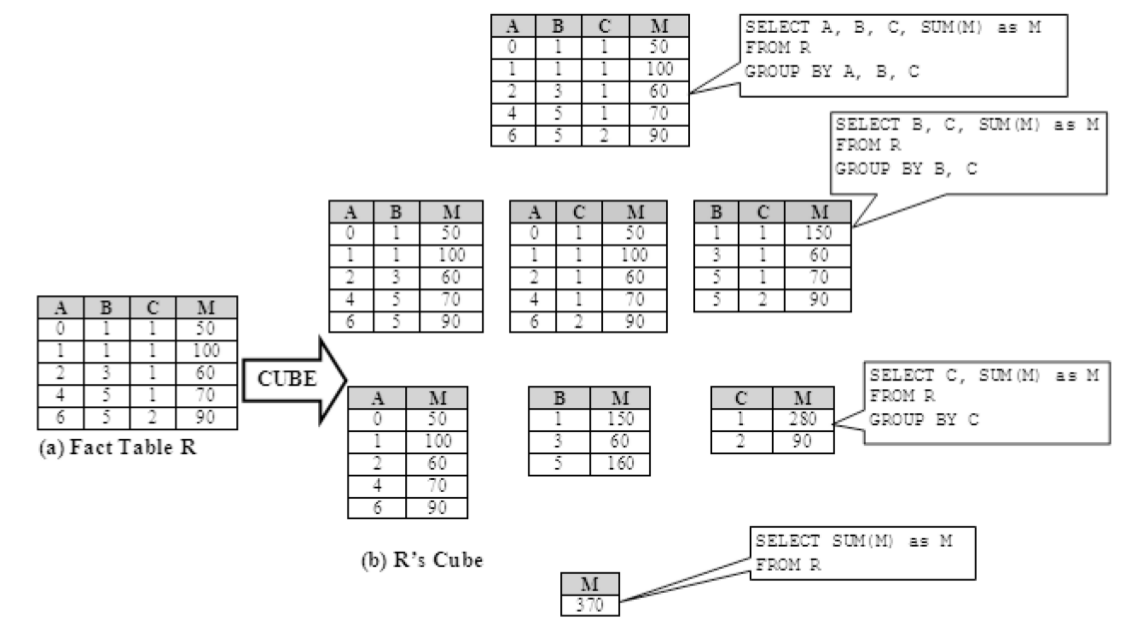
\includegraphics[width=6in]{picture/ch_preliminary/fact_table_data_cube} 
\caption{事实表与数据立方}\label{fact_table_data_cube} 
\end{figure} 

\section{Lattice, Region, Group}

对于图\ref{fact_table_data_cube} 中的所有GROUP BY,可用另一种方式表示,如图\ref{abc_lattice} 所示,这种结构称为 Lattice。

\begin{figure}[hbtp]
\centering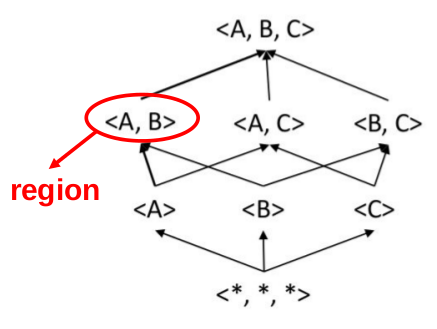
\includegraphics[width=2in]{picture/ch_preliminary/abc_lattice} 
\caption{ABC Lattice}\label{abc_lattice} 
\end{figure} 

在这个lattice中,有维属性对应的所有 GROUP BY 类型,每个节点表示一种 GROUP BY 类型,箭头连接的两个节点表示它们有父子关系。在lattice中的每个节点又称为一个Region,也就是一种 GROUP BY 类型。一个 region 内有多个 group。group 指的是一个
Region中带有具体值的 Group By。例如图\ref{fact_table_data_cube} 中的 GroupBy(A),就有表\ref{groupby_a_table}的结果。

\begin{table}[hbtp]
\begin{center}
\begin{tabular}{|c|c|}
\hline 
A & M \\ 
\hline 
0 & 50 \\ 
\hline 
1 & 100 \\ 
\hline 
2 & 60 \\ 
\hline 
4 & 70 \\ 
\hline 
6 & 90 \\ 
\hline 
\end{tabular} 
\end{center}
\caption{GroupBy(A)}\label{groupby_a_table}
\end{table}

在表\ref{groupby_a_table}中,Region \textless A\textgreater 中有5个Group,分别是Group(A=0), Group(A=1), Group(A=2), Group(A=4), Group(A=6)。

从lattice中可见,当一个事实表有 D 个维属性时,它对应的数据立方就会有${2}^{D}$个region,也即有 ${2}^{D}$ 种不同类型的 GROUP BY 的查询。最简单直接(Naive)的数据立方实现方法,会对每个region进行独立计算并把结果存储起来。对于一张事实表,随着他的维属性数量的增加,它相对应的数据立方的计算与存储代价就会呈指数增长。于是,在 ROLAP 中,如何从立方计算、立方存储这两个角度高效地实现数据立方已成为业界内广泛讨论的一个研究课题。


\section{度量}

度量,即对GROUP BY的多条数据进行计算,例如SUM,AVEG,MEDIAN等。

度量函数一般分为三大类, 分别是分布式度量(Distributive),线性度量(Algebraic)和整体性度量(Holistic)。

以下使用一个二维的数据集$\left\{ {X}_{ij}|i=1,...I; j=1,...J \right\}$分别说明这三种度量函数的区别。

\begin{itemize}

\item \textbf{分布式度量}

对于分布式度量函数 F(),如果存在一个辅助函数 G() 能令 $F(\text\{ {X}_{i,j} \text\}) = G(\text\{ F(\text\{ {X}_{i,j}|i=1,...,I \text\})|j=1,...J \text\})$,则度量函数 F() 为分布式度量函数。常见的分布式度量函数有 COUNT(), MIN(), MAX(), SUM()。大部分分布式度量函数中 $F=G$,但COUNT() 除外。在COUNT()度量函数中,$G=SUM()$。

\item \textbf{线性度量}

对于线性度量函数 F(),如果存在辅助两个函数 G() 和 H(),其中 G() 的输出结果是确定数量固定的 M 条记录,并且满足$F(\text\{ {X}_{i,j} \text\}) = H(\text\{ G(\text\{ {X}_{i,j}|i=1,...,I \text\})|j=1,...J \text\})$。常见的线性度量函数有Average(),MaxN(),MinN(),standard deviation等。例如对于Average(),函数G()的输出是子集的和以及数量,H()函数则把将各个子集的和相加再除以数量的总和。线性度量的关键是,函数G()的输出结果的数据多少是确定的。例如Average(),无论数据怎么划分,函数G()的输出都是两个数,一个是和,另一个是数量。

\item \textbf{整体性度量}

对于整体性性度量函数 F(),其中间结果,即各个子集的计算结果的数据量大小是不确定的。常见的整体性度量有Median(), Mode(), RANK(), DISTINCT()等。

\end{itemize}

之所以要对度量函数进行分类是因为其会影响数据的划分。论文研究的是分布式环境下数据立方的计算,因此数据划分是必然的。对于以上三种度量,在分布式度量与线性度量下,数据无论如何划分,使用辅助函数都能计算出最终结果,并且中间结果的数据大小是确定的。但对于整体性度量,虽然数据不能随意划分,或者数据的随意划分对其计算的意义并不大,但并不代表数据不能划分。在后面的章节中会提到,对于整体性度量按照一定的方法对数据进行划分,也能令中间结果的数据大小是确定的。

\section{MapReduce}

MapReduce是Google提出的一个软件架构,用于大规模数据集的并行运算。MapReduce的数据流动如图 \ref{mr_data_flow} 所示。它的整个执行流程分为以下几个步骤:

\begin{enumerate}
\item 输入的数据被划分成块分派到各个Map任务中。
\item Map对输入的数据块处理后,排序并写到磁盘上,输出格式为键值对(Key-Vavlue)。
\item 在Merge阶段从各个Map获取具有相同Key值的数据。
\item 在Sort阶段,将上一阶段合并的结果排序后发到对应的Reducer上。
\item Reducer对输入的键值对进行处理后输出。具有相同Key值的数据会被分派到同一个Reducer任务上。
\end{enumerate}

\begin{figure}[hbtp]
\centering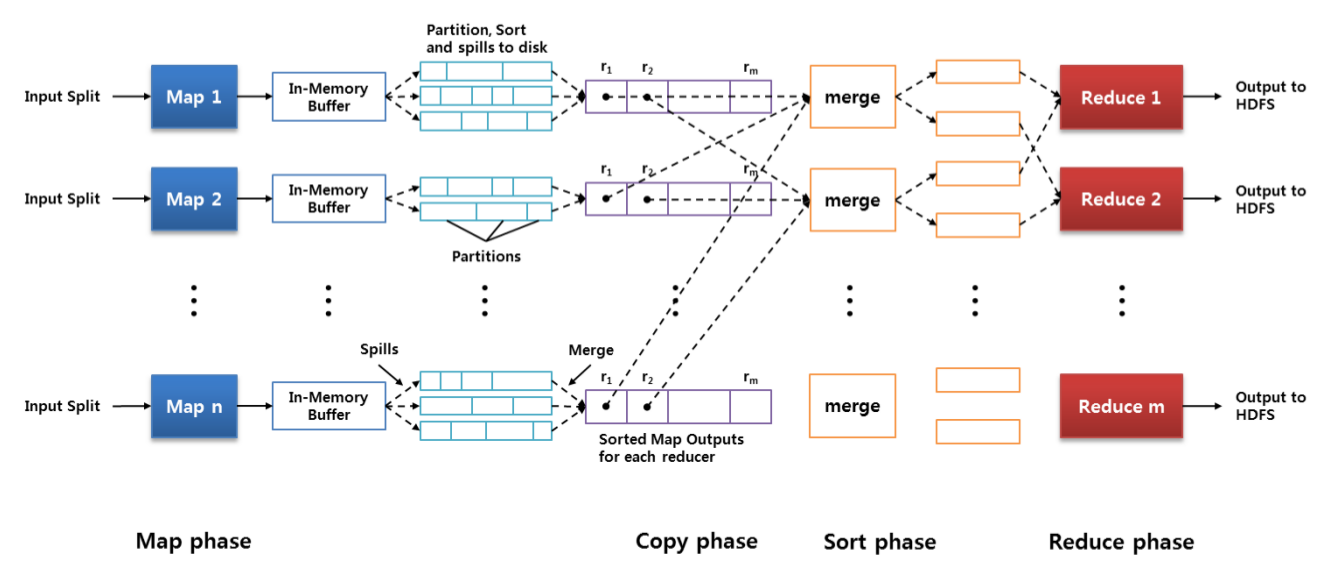
\includegraphics[width=6in]{picture/ch_preliminary/mr_data_flow} 
\caption{MapReduce的数据流动}\label{mr_data_flow} 
\end{figure} 

图\ref{mr_word_count}是用MapReduce进行单词统计的例子。

\begin{figure}[hbtp]
\centering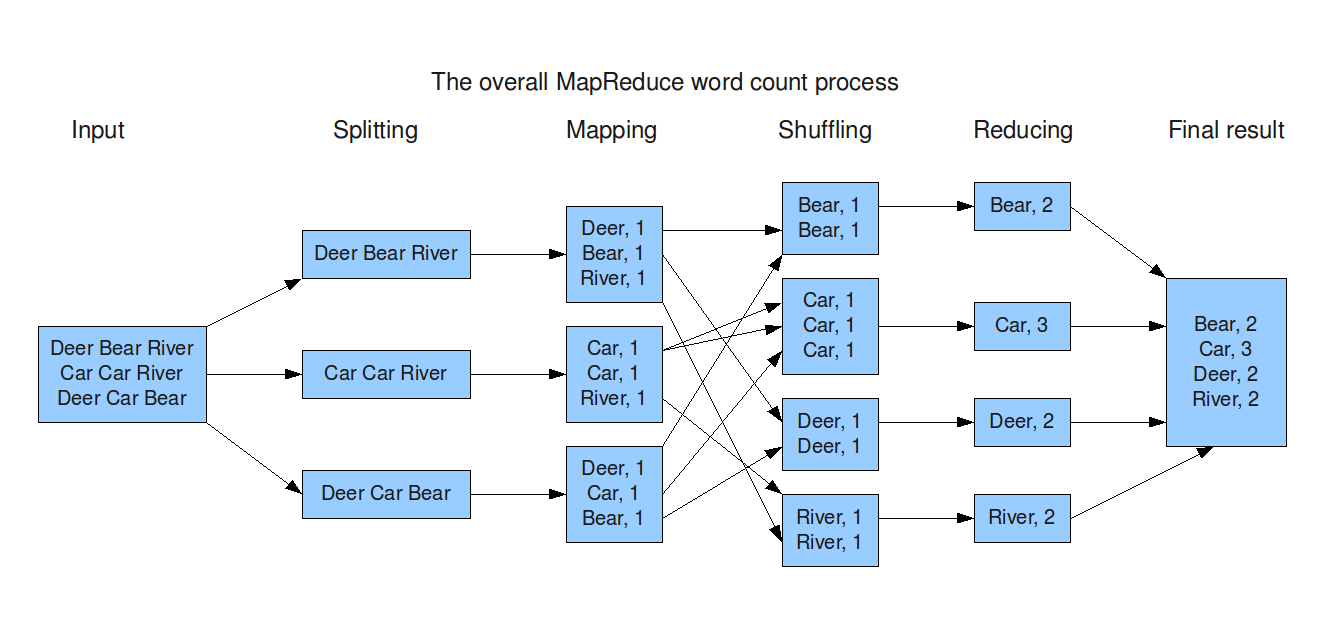
\includegraphics[width=6in]{picture/ch_preliminary/mr_word_count} 
\caption{MapReduce单词统计例子}\label{mr_word_count} 
\end{figure} 




\chapter{相关研究现状分析}


\section{数据立方的计算研究}

数据立方的计算涉及到对原事实表数据进行扫描,对相应的 GROUP BY 属性值执行聚合计算以及生成相应的立方数据等几个步骤。在立方计算的问题讨论中,如何尽可能地减少原事实表的数据扫描次数、降低 I/O 代价以及计算过程中内存的开销,成为评价一个立方计算方法高效性的几个关键要点。

GBLP \cite{gray1997data}、PipeSort、PipeHash \cite{agarwal1996computation}、BUC \cite{beyer1999bottom} 以及 Partitioned-Cube \cite{ross1997fast} 是几种经典的数据立方计算方法。 其中GBLP、 PipeSort、 PipeHash以及Partitioned-Cube 均是自顶向下的计算,而 BUC 则是自底向下的计算方法。如图 \ref{4_dimension_lattice},展示了一个 4 维数据立方的 lattice,其中 A,B,C,D 均为属性维度。在一个数据立方 lattice 中,每一个节点代表一个数据小方,箭头从父节点指向子节点。自顶向下,顾名思义就是在一个 lattice 中从父节点开始往下计算,而自底向上则相反。

\begin{figure}[!htb]
\centering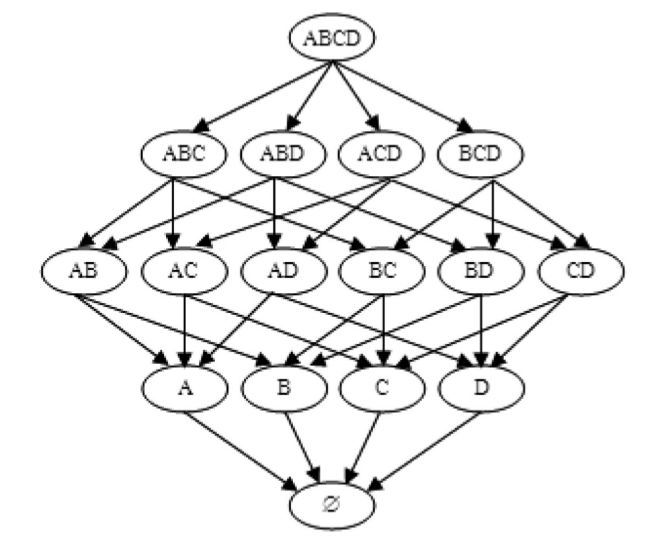
\includegraphics[width=3in]{picture/ch_current_research/4_dimension_lattice} 
\caption{4维数据立方的Lattice}\label{4_dimension_lattice} 
\end{figure} 

\begin{itemize}

\item \textbf{GBLP}

Jim Gary 等人在提出数据立方概念的同时,还提出了一种计算数据立方的算法 —— GBLP[12]。该算法的核心思想是自顶向下,为每个小方选择其最小的父小方(指小方内group数量最少)作为其计算的基础。对于一个立方 lattice,越往下,小方内group的数量就会变得越少,因此相对于每个小方都基于原始数据表进行计算,基于最小父小方的计算,因为数据量的大规模减少而加快了一个小方的计算速度。但该方法只是把一个 lattice 修剪成一个树型结构,却没有提供一个特定的 lattice 树遍历计划。另外当计算数据量很大无法完全存储于内存时,该方法没有提供一个有效的磁盘访问策略而使得 I/O 代价会很高。

\item \textbf{PipeHash}

1996 年,Agrarwal 等人针对 GBLP 算法的缺陷,提出了第一个改进的数据立方计算方法 —— PipeSort\cite{agarwal1996computation} 。在一个数据立方 lattice 中,假如一个子小方的维属性排序顺序是它其中一个父小方的维属性排序顺序的前缀,则该子小方可以在其父小方的基础上计算而无需额外的排序。如前面提到的图 2 所示的数据立方,假设每个小方的维属性排序顺序就是图示的小方名字从左到右的维顺序,例如对于小方 ABC,首先按照维属性 A 排序,若 A 相同的情况下再按照 B 排序,以此类推。小方 AB 的维顺序是小方 ABC 的前缀,但小方 AC 不是小方 ABC 的前缀。在这样的情况下,AB 可从 ABC 计算获得,ABC 可从 ABCD 计算获得,于是形成了流水线 ABCD-\textgreater ABC-\textgreater AB-\textgreater A。因此对原数据和一些小方进行多次排序,即可生成多条流水线。

PipeSort 在 GBLP 的基础上,通过采样估算每个小方的大小,通过二分匹配的方法找出每个子小方需要从哪个父小方计算获得。然后基于这个二分匹配的结果将一个 lattice 切割成多棵子树,称为 pipeline (流水线),pipeline 内只有根节点需要对输入数据进行排序。对于每个 pipeline,从根节点逐层往下计算,除根节点外,只需在内存中为每个节点缓存一条元组,极大的提高了内存的使用率。只是,当数据立方的维度变得很高时,PipeSort 的排序代价则会成指数增长。 且当数据比较稀疏时,排序的中间结果不能完全存储于内存中,还需进行外部排序,增加了 I/O 代价。图\ref{pipesort} 为 4 维数据立方使用 pipesort 的计算过程。图(a)中的虚线表示从父小方排序后得到子小方的过程,实线表示流水线的计算过程。图(b)是最终需要计算的流水线,椭圆中的小方表示需要重新排序。

以上提到的几种算法都没有考虑到数据稀疏的情况,在现实应用中,事实表往往是稀疏的。针对基于稀疏基表的数据立方的有效计算 ,Ross 等人在1997 年提出了 Partitioned-Cube 算法[20]。该算法采用分治的策略,对不能完
全存储与内存的数据集根据某个候选聚集维属性进行划分,划分成多个子集,
因为数据是稀疏的,所以能使得每个子集均能在内存中计算,于是通过此次划
分能够计算所有和该维属性相关的小方结果。完成计算后,将该划分维从候选
聚集维中去除,根据上述方法重复计算基于剩余维属性的小方结果直至立方计
算完毕。相对于前几种算法,这种算法在数据稀疏的情况下具有更小的 I/O 代
价,且受维度增加的性能影响较少。

\begin{figure}[!htb]
\centering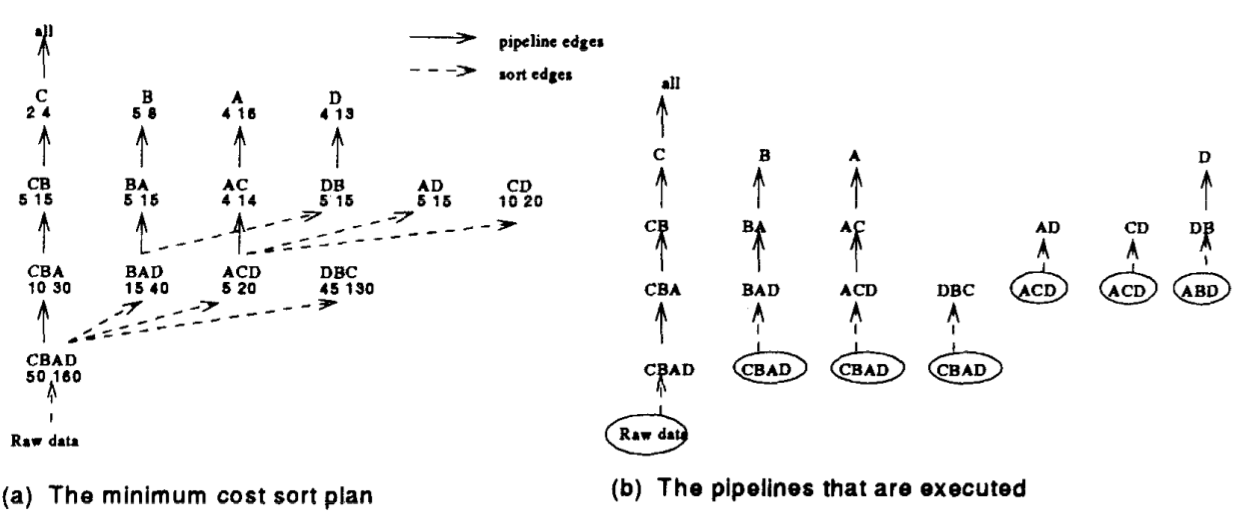
\includegraphics[width=5in]{picture/ch_current_research/pipesort} 
\caption{4维数据立方 pipesort 计算过程}\label{pipesort} 
\end{figure} 

\item \textbf{PipeHash}

Agrarwal 等人还提出了 PipeHash[19]算法,该算法是 PipeSot 算法的一个变形,基于 Hash(散列)实现的。PipeHash 算法首先会根据 GBLP 算法的思想将一个立方 lattice 修剪成一棵 lattice 执行树。为了使得在同一个聚集计算里的所有元组能够在内存上相邻的位置,PipeHash 会为每一个同时计算的小方维护一个 Hash 表。假如有些小方的散列表不能同时存放在内存里,则 PipeHash 算法就会把一个 lattice 执行树划分成多棵子树,使得每棵子树内所有小方的 Hash表都能够同时存储于内存中。 由于划分代价要比排序代价要小,所以PipeHash 的性能要比 PipeSort 要高。但 PipeSort 用一个排序可以计算多个聚集结果,而 PipeHash 则每次都需要对数据进行重新 Hash,且 PipeHash 相对于PipeSort 需要大量的内存来存储每棵子树内所有小方的 Hash 表。

\item \textbf{Partitioned-Cube}

以上提到的几种算法都没有考虑到数据稀疏的情况,在现实应用中,事实表往往是稀疏的。针对基于稀疏基表的数据立方的有效计算 ,Ross 等人在1997 年提出了 Partitioned-Cube 算法 \cite{ross1997fast}。该算法采用分治的策略,对不能完全存储于内存的数据集根据某个候选聚集维属性进行划分,划分成多个子集,因为数据是稀疏的,所以每个子集均能在内存中计算,于是通过此次划分能够计算所有和该维属性相关的小方结果。完成计算后,将该划分维从候选聚集维中去除,根据上述方法重复计算基于剩余维属性的小方结果直至立方计算完毕。相对于前几种算法,这种算法在数据稀疏的情况下具有更小的 I/O 代价,且受维度增加的性能影响较少。图\ref{partitioned_cube} 为 4 维数据使用 Partitioned Cube计算的过程。

\begin{figure}[!htb]
\centering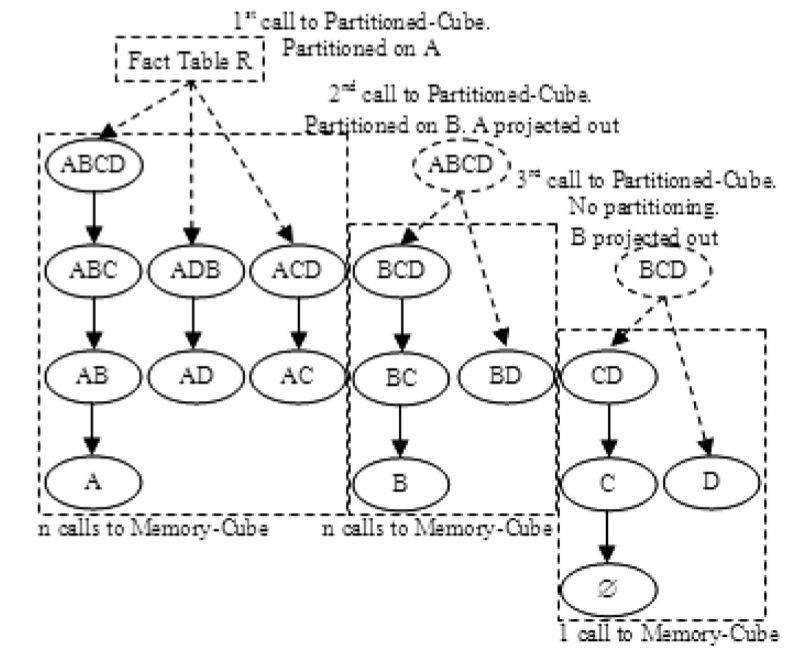
\includegraphics[width=3.5in]{picture/ch_current_research/partitioned_cube} 
\caption{Partitioned Cube 的计算过程}\label{partitioned_cube} 
\end{figure} 

\item \textbf{BUC}

相对于上述几种自顶向下的立方计算算法,Beyer 等人在 1999 年提出的 BUC (Bottom Up Cube) 则是一种自底向上的算法。BUC 算法是在 Partitioned-Cube 算法的思想上,针对冰山数据立方,即基于某个最少阈值的 GROUP BY 计算而提出的,也即具有 HAVING 条件的 GROUP BY。例如 HAVING COUNT(*) > 100 这样的条件限制。大部分的度量函数是具有单调性的,例如 COUNT(),若 GROUPBY(A=a0) 的结果是小于 100,那么 GROUPBY(A=a0, B=b0) 的结果必然是小于 100。正是这种单调性,加上有阈值限制,将数据立方的计算变成从底向上,可以实现一定的剪枝。例如上述的例子 COUNT(*) > 100,如果 GROUPBY(A=a0)是小于 100 的,那么与 A=a0 相关的 group 就不需要计算了。

BUC算法会根据聚集维属性对基表数据进行多次分组并计算聚集结果,并会基于维顺序对分组进行进一步的细分计算。因为在计算过程中考虑了阈值的问题,所以从 lattice 的底部越往上,小方需要进行聚集计算的数据就会变得越少。由于 PipeSort,PipeHash,PartitionedCube 在计算稀疏数据立方时都会产生相对较大的 I/O 和内存消耗代价,所以 BUC 算法在计算稀疏矩阵时的性能要比以上几种算法性能要好。图 \ref{BUC_partition} 是 BUC 根据属性 A 进行的划分。图 \ref{BUC_execution} 是 BUC 的执行过程。在图 \ref{BUC_execution} 中,原数据分别按照 A, B, C, D 这4个属性进行划分。在属性 A 的划分中,计算所有与属性 A 相关的数据小方,当出现一个小方不满足阈值时,则往上的小方都不需要计算了。

\begin{figure}[!htb]
\centering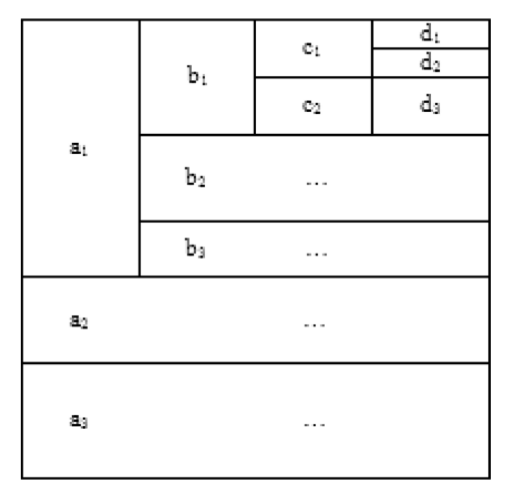
\includegraphics[width=1.7in]{picture/ch_current_research/BUC_partition} 
\caption{BUC 使用维属性的划分}\label{BUC_partition} 
\end{figure} 


\begin{figure}[!htb]
\centering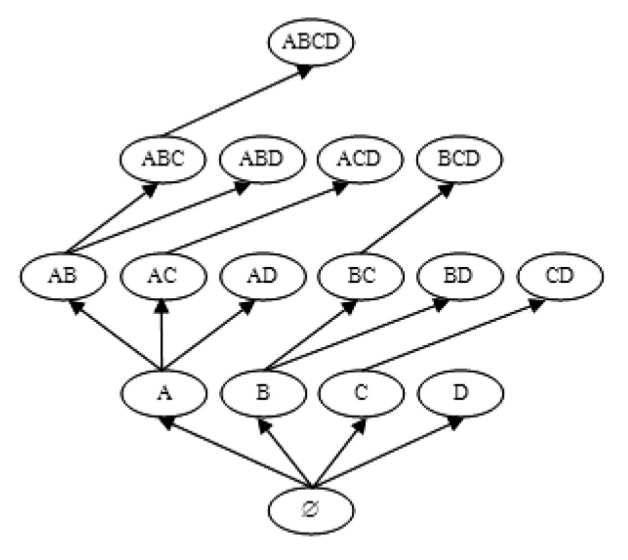
\includegraphics[width=3in]{picture/ch_current_research/BUC_execution} 
\caption{BUC 的执行过程}\label{BUC_execution} 
\end{figure} 

\end{itemize}

\section{部分数据立方的计算研究}

在前文提到,当一个数据立方的维度为 D 时,数据立方内就包含了 ${2}^{D}$ 个数据小方,也即 ${2}^{D}$ GROUP BY 计算。当维度增加时,数据立方的计算和存储代价就会呈指数增长。在现实条件下,计算时间和存储空间往往都受限制,而且对于某些数据小方,在现实中也常常不是 OLAP 分析人员需要的数据。因此可选择只计算部分的数据立方,在这里提到的部分数据立方,是指在立方实现与存储时选择了部分小方而非所有小方的数据立方。当查询的数据小方已经计算了,则可直接查询获得;若查询的数据小方未计算,则从已计算的数据小方中计算获得,而非原数据。于是,如何合理的选择部分立方进行计算就成了部分数据立方计算实现和查询相应速度的关键。

Harinarayan 等人在1996 年提出的贪心算法 BPUS \cite{harinarayan1996implementing} ,通过单位空间效益的指标来对小方节点进行贪心选择。该算法比穷尽搜索要快,但算法复杂度较高,随立方维度增加算法时间复杂度呈指数增长。 Shukla等人在 1998 年基于 BPUS 算法思想提出了一个使用简单启发式搜索的改进算法 PBS \cite{shukla1998materialized} ,该算法时间复杂度较低其运行速度比 BPUS 要快几个数量级,且它能够容易的与自底向上的立方计算方法整合,但该算法会为了加快其运行速度而牺牲了一定的结果质量。除了以上几个贪心算法外,业界也提出了其他的优化贪心算法来进行小方选择。同时,除了从存储代价角度来考虑立方选择之外,业界也尝试从立方维护代价等多个角度进行小方选择算法的设计与优化。

\section{分布式数据立方的计算研究}

随着计算量的极速增长,对于 OLAP 技术中的关键技术 —— 数据立方,业界也开始研究利用分布式计算的优势实现数据立方的方法。\cite{nandi2011distributed} \cite{dehne2006cgmcube} \cite{ng2001iceberg} \cite{lee2012efficient}。

\cite{ng2001iceberg} 中提出了在由一定数量的 PC机 组成的集群上计算数据立方的方法,包括了RP、BPP、ASL、PT。因为该论文提出的实现环境是集群,因此这4种方法都涉及如何将计算分配到多个节点上。以下简单地阐述这4种方法。

\begin{itemize}

\item \textbf{RP(Replicated Parallel BUC)}

RP 对计算的划分非常简单,基本与 BUC 相似,若有 m 个维属性,则将计算划分为 m 个子任务。每个任务处理与一个维属性相关的所有小方的计算。如图 \ref{cluster_rp} 所示,图中因为共有 4 个维属性 ABCD,因此可将计算划分为 4 个子任务,分别计算从维属性 A,B,C,D 出发的各个数据小方。

\begin{figure}[!htb]
\centering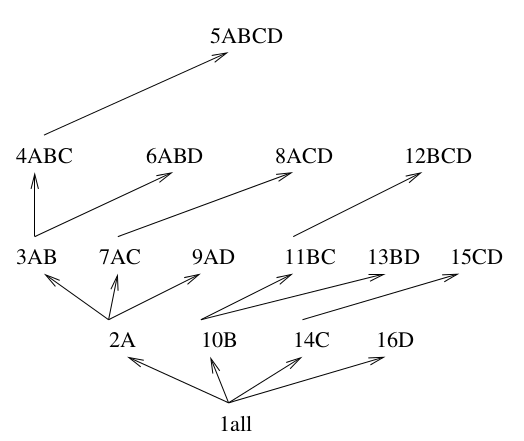
\includegraphics[width=3in]{picture/ch_current_research/cluster_rp} 
\caption{RP 的任务划分图}\label{cluster_rp} 
\end{figure} 

\item \textbf{BPP(Breadth-first writing, Partitioned, Parallel BUC)}

RP 的划分非常简单,同时也存在非常严重的负载均衡问题,有一些任务需要进行大量的计算,如图 \ref{cluster_rp} 中的维属性 A 对应的任务,而有一些则只需要进行非常少量的计算,如 D。BPP 则可以解决该问题。BPP 借鉴了 \cite{ross1997fast} 中的 Partitioned-Cube 算法。

对于一个属性 ${R}_{i}$,根据其属性值的范围,将数据集划分为 n 个子块,而 n 正是节点的数量。对于每个属性都进行类似的划分操作。因此,若有 m 个维属性,则有 $n \times m$ 个子块。多个属性的子块划分可同时进行,最后将这些子块分发到各个节点上计算相应的数据小方。

这样的方法比 RP 相比,负载均衡的问题就减轻不少。

\item \textbf{ASL(Affinity SkipList)}

ASL 使用跳表来维护小方内的数据。跳表的一个重要特征是其有序性。因此若对数据小方 ABCD 维护了一张跳表,则可从调表上计算 ABC,AB,A 这三个数据小方。这个与 Pipesort 类似。若要计算的小方并没有建立跳表,但它是已建立跳表的小方的后缀,则仍可从已建立的跳表中较快速地计算。如小方 BCD 可从 ABCD 中计算获得,相比从原数据中计算获得有更高的效率。如果以上两种情况都不满足,只能重新构建跳表。
 
\item \textbf{PT(Partitioned Tree)}

PT 是对 lattice 不断使用二分划分的方法,直到划分的子 lattice 的数量与节点数量相同则停止。图 \ref{cluster_pt} 是 PT 的任务划分图。

\begin{figure}[!htb]
\centering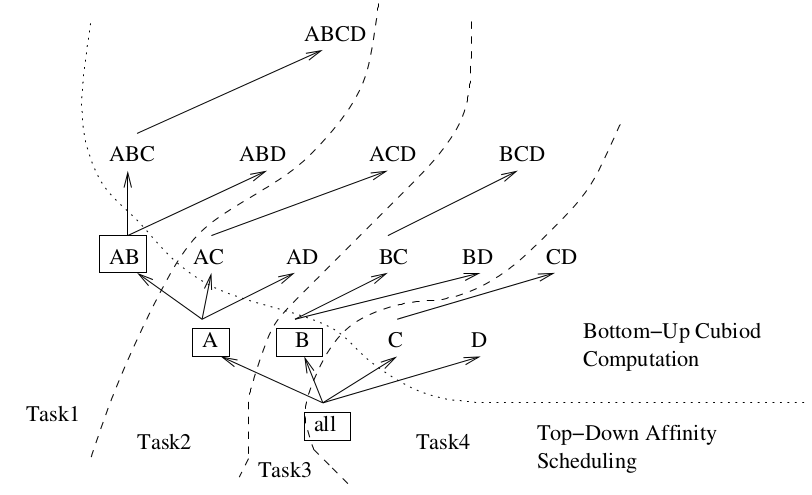
\includegraphics[width=4in]{picture/ch_current_research/cluster_pt} 
\caption{PT 的任务划分图}\label{cluster_pt} 
\end{figure} 

\end{itemize}


cgmCUBE \cite{dehne2006cgmcube}、RP、BPP、ASL、PT\cite{lee2012efficient} 这几个算法是基于由少量 PC 机组成的集群实现的,无法适应 TB 级的处理数据量,也并没有与 MapReduce 框架相结合。 \cite{you2008parallel} \cite{sergey2009applying} 虽将数据立方的计算与 MapReduce结合,但无法很好地处理整体性度量函数的计算,也并没有考虑到数据倾斜的情况。

MR-Cube[5][14]是基于 MapReduce 提出的数据立方算法,该算法结合了 MapReduce 与数据立方计算的特点,能够达到高效实现 TB 级数据量的数据立方计算。MR-Cube 针对整体性度量函数提出了相应的分布式计算思路,并指出了其中 2 种整体性度量函数实际的分布式计算处理方法。 为了避免MapReduce 集群节点间的数据分布不均衡,MR-Cube 采用对基表进行采样的方法来决定如何在后续计算中对数据小方进行切割以使得集群节点间的装载平衡。利用数据立方小方间计算过程可共享的特性, MR-Cube 对原数据立方lattice 进行分支,使得每个分支能在共享一套数据的基础上进行 BUC 计算,从而降低了 MapReduce 的中间处理数据量。

虽然 MR-Cube 是目前基于 MapReduce 框架一个较好的数据立方实现尝试。但与此同时,MR-CUBE 现有的一些不足不得不提。MR-Cube 的数据切割是基于整个数据小方的,当数据小方内某个元组的计算数据过度倾斜,而其他元组的计算数据都较小时,对整个数据小方进行切割就会导致一些元组不必要的切割。过多的切割会导致后续的合并计算过多,当数据过度倾斜时,这种切割方式的劣势就会显得十分明显。并且在 lattice 分支上使用 BUC 的计算,没有充分利用 MapReduce的特性,BUC 需要对数据扫描多次,这样导致多次I/O或者需要将数据都载入内存。

由于本文的主要工作是对 MR-Cube 进行改进,因此关于 MR-Cube 主要的贡献和存在的不足将在下一章详细说明。




\chapter{MR-Cube 实现分析}

本章节中将对 \cite{nandi2011distributed} 中提出的 MR-Cube 进行具体分析,包括它的主要贡献和存在的不足。

\section{数据集}

在接下来的章节中需要数据集作为例子,因此首先介绍作为例子的数据集,这里使用\cite{nandi2011distributed}  中的数据集。数据集的表结构如图 \ref{dataset_table} 所示。表中数据记录的是不同地区的用户的查询记录。属性id为表的主键,记录每条记录的id;time为查询时间;uid为用户的id。表中剩余的 6 个属性为维属性,分别是 country,state,city,topic,category,subcategory。country,state,city 记录地区信息,topic,category,subcategory 记录查询内容。其中\textless country, state, city\textgreater 是具有层次型的,同理\textless topic, category, subcategory\textgreater 也是具有层次性的。因此在 GroupBy 时,GroupBy(country, state, topic) 和 GroupBy(state, topic)是等价的。并且不会出现 GroupBy(country, city, topic) 这样的跨越层次的操作。

该数据集对应的 lattice 如图 \ref{dataset_lattice} 所示。图中的 ``*" 表示不需要聚合的属性。因为数据集具有层次型,因此lattice与上一章中看到的有所不同。上一章中提到,若有 D 个维属性,则 lattice 中有${2}^{D}$ 个节点,但由于这个数据集具有层次型,因此节点数有所减少。例如对于 (country, state, city) 这3个属性的 GroupBy,仅有 3 种结果,即 GroupBy(country),GroupBy(country, state)(或 GroupBy(state)) 以及 GroupBy(country, state, city)(或 GroupBy(city))。因此该数据集对应的lattice中共有16个region,也就是该数据集共有16种 GroupBy 类型。


\begin{figure}[!htb]
\centering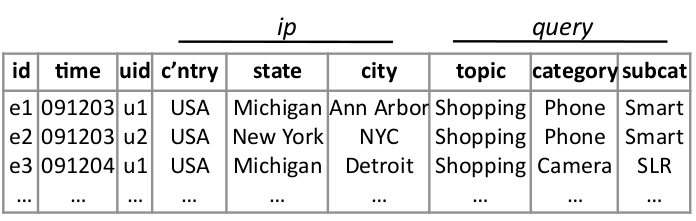
\includegraphics[width=3.5in]{picture/ch_datacube_mr/dataset_table} 
\caption{数据集的表结构}\label{dataset_table} 
\end{figure} 

\begin{figure}[!htb]
\centering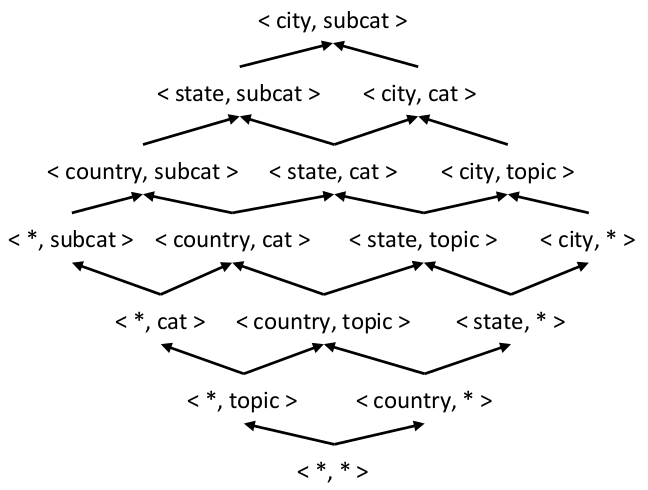
\includegraphics[width=3in]{picture/ch_datacube_mr/dataset_lattice} 
\caption{数据集的lattice}\label{dataset_lattice} 
\end{figure} 

\section{Naive 算法}

算法 \ref{naive_algorithm} 为使用 MapReduce 计算数据立方的 Naive 实现。例如上述的数据集共有16个 region,那么对于输入的每一条记录,将其映射成对应的所有 group,并且与度量属性的值组成 key-value 作为 mapper 的输出。相同 key 值的数据将分派到同一个 reduce 函数中,也即相同 group 值的数据被分派到同一个 reduce 函数中,再进行聚合计算。例如输入的一条记录为 (e1, 091203, u1, USA, New Youk, NYC, Shopping, Phone, Smart),度量函数为 COUNT(DISTINCT(uid)),该度量函数是计算group内有多少不同的uid。那么对于每一条记录,map 都输出 16 个 ([group value], [uid]) 的key-value,分别为([*,*], [u1]), ([*,Smart], [u1]), ([USA, *], [u1])等等。reducer 再对同一个 group 内的数据进行聚合计算。

{\renewcommand\baselinestretch{1} 
\begin{algorithm}[!ht]
\caption{Naive Algorithm}
\label{naive_algorithm}
{\fontfamily{\familydefault}\selectfont

	\begin{algorithmic}[1] %每行显示行号
    \Function {MAP}{e}
    	\State e is a tuple in the dataset
        \ForAll {Region R in C}
        	\State k=R(e)
        	\State EMIT([k], [e])
        \EndFor
   	 \EndFunction
     \State
     \Function {REDUCE}{k,$\left\{ e1,e2,...\right\}$}
     	\State let M be measure function
        \State EMIT(k, M($\left\{ e1,e2,...\right\}$))
     \EndFunction
	\end{algorithmic}
}
\end{algorithm}
\par}

Naive的方法实现起来非常简单,对于较小的数据集也有很好的效果,但是随着数据集规模的增大,Naive方法的不足则非常明显,主要包括以下两个方面。

\begin{itemize}

\item \textbf{中间数据过多}

若 lattice 中的 region 数量为 $|C|$,数据集的大小为 $|D|$,则中间数据的数据量为 $|C|\times |D|$。随着维属性数量的增加,与层次的加深,中间数据的数据量则会巨增,必然导致 map 阶段有大量的磁盘 I/O,以及 shuffle(sort) 阶段有大量的数据需要排序,对整体的效率有非常大的影响。

\item \textbf{超大group}

在 MapReduce 计算中,总体的计算时间是由计算时间最长的 reducer 决定。因此若各个 reducer 分配到的要计算的数据量差异较大时,会导致某些 reducer 运行时间远大于其他 reducer。 在 Naive 的计算方法中,具有相同 group 值的数据会在一个 reducer 中计算,当一个 group 很大时,例如 lattice 中处于底层的 region 中的 group 相对就会较大,它运行的时间就会很长,而其他处理小 group 的 reducer 因为较早处理完数据,可能会空闲等待,甚至重新启动大 group 的计算,但重启计算效果往往并不佳,最终导致整个 MapReduce 的计算时间过长。

\end{itemize}

以上两个不足,主要出现在整体性度量函数的计算中,而对于代数度量函数,例如SUM,COUNT,AVG 等,则不会有以上的问题。因为MapReduce的combiner机制与代数度量函数的计算有非常好的整合。combiner 是 MapReduce 一个重要的机制,它等同于本地的 reducer。它会对 mapper 的输出进行一次本地的 reduce 计算,然后再将数据发到相应的 reducer 上,这样可以减少网络传输的数据量和reducer 的计算量。正因为这个 combiner 的作用,对于代数度量函数,combiner 可以在本地对同一个 group 内的数据进行一次计算,将一个 mapper 上同一个 group 内的数据压缩成一条记录发送给 reducer,而不是将这个 group 内的数据直接发送到 reducer上,这样每个 reducer 获得的数据量比不使用 combiner 获得的数据量要少得多。由于mapper的数量是有限的,那么分发到一个reducer上一个group内的数据也是有限的。这样有限的数据必然不会导致中间数据过多和各个reducer上数据的不均匀。实验部分也会对这两种度量进行比较。

但是对于整体性度量函数,combiner的作用却可能很小,这也是整体性度量函数与代数度量函数最大的区别,因为整体性度量函数中间结果的数据量是不确定的。例如对于COUNT(DISTINCT(uid))的计算,combiner可将同一个group内多条具有相同uid的记录压缩成一条输出,若uid取值较多,甚至无重复,则combiner几乎无法发挥作用。那么就会出现以上提到的两个问题。针对这两个问题,MR-Cube提出了相应的解决方案。

\section{MR-Cube}

\subsection{整体性度量的划分}

对于大 group 的问题,可以将一个大 group 划分成多个子 group,将这些子 group 分发到多个 reducer 上计算,即可解决 reducer 计算数据量不均匀的问题。

对于代数度量函数,数据是可以随意划分的。但是整体性度量函数的划分就没有这么简单了。例如整体性度量函数 COUNT(DISTINCT(uid)),它是计算不同的 uid 的数量。如果对数据集进行随意的划分,每个子块的计算结果是不同的 uid 列表,即对子块中相同的uid只保留一个。然后再对这些 uid 列表进行统计计算 COUNT(DISTINCT(uid))。这里每个子块的计算结果不能是COUNT(DISTINCT(uid)),这样会导致最终结果是错误的。中间结果是不同的 uid 列表,如果 uid 重复度非常高,那么各个列表中uid的数量较少,这种划分计算方法是可行的。但倘若 uid 的重复度非常低,各个列表的uid很可能跟子块中uid数量同样多,那么这种随意划分的方法则毫无作用。 

因此 MR-Cube 的论文中给出了一种对整体性度量函数进行划分的方法,称为部分代数度量 (Partially Algebraic Measure)。例如对于 COUNT(DISTINCT(uid)) 的度量计算,数据可按照 uid 进行划分,那么具有相同 uid 的记录会被划分到同一个子块中,而每个子块之间的 uid 是不会有相同的。这样对于每个子块都可以输出一个整数,即该子块 COUNT(DISTINCT(uid)) 的结果,最后将各个子块的结果相加即可得到最终结果。论文中将 uid 这样的用来划分的属性称之为代数属性。这样的划分方式对于很大部分的整体性度量都是有效的,例如TopK,MODE等。


\subsection{Reducer-Unfriendly Group}

确定了数据的划分方法,下一个问题是哪些 group 需要划分,也就是哪些 group 是较大的 group。在论文中使用了随机均匀采样的方式选取部分的数据进行数据立方的计算,在每个 group 内做 COUNT,也就是统计每个 group 的大小,然后根据数据集大小、采样数量、reducer limit(根据内存大小估算reducer可处理的数据量)以及使用切诺夫界确定一个 group 是否是 reducer-unfriendly group。用直观的理解即是,通过概率统计的方式确定采样中的 group 是否是较大的 group,这些 group 被称为 reducer-unfriendly group。并且对于 unfriendly 的 group,会根据group的大小以及reducer limit 估算出划分因子。对于划分因子的直观理解,即是这样一个大 group 应该划分多少子块,才能令每个子块不超过 reducer 处理数据量的上限。

若一个 region 中有一个 group 是 reducer-unfriendly 的,那么这个 region 也就是 reducer-unfriendly 的。在采样后的正式计算中,对于 reducer-unfriendly region 内的所有 group 都需要进行划分。划分的方式使用上一节中提到的对整体性度量的划分方式,即根据某一个代数属性,如 uid 进行划分。如图\ref{region_partition}所示,根据采样的结果将region划分成了 friendly 和 unfriendly 两类。对于 unfriendly 的 region,region 内的所有 group 都需要划分,论文中使用求余方式进行划分。

\begin{figure}[!htb]
\centering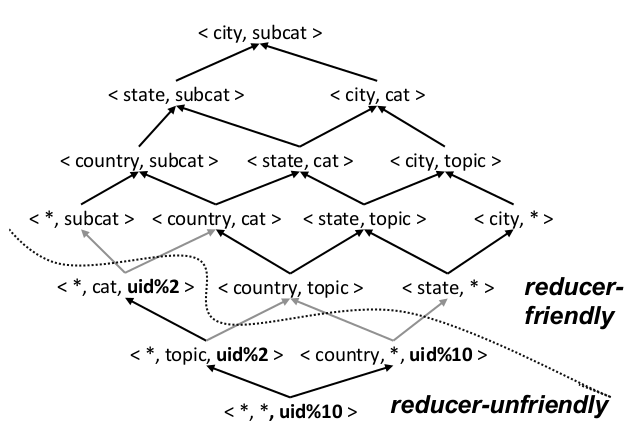
\includegraphics[width=3.5in]{picture/ch_datacube_mr/region_partition} 
\caption{根据uid被划分的lattice}\label{region_partition} 
\end{figure} 

上述的方法只记录需要划分的region,这是因为 region 的数量远比 group 少得多。若要记录所有的需要划分的 group,则需要太大的开销。只记录region的方法能保证大 group 的划分,但是如果 region 中只有 1 个 group 是 unfriendly 的,其他的friendly 的 小group 也要被迫划分,这样将导致不必要的划分以及出现过多的被划分数据,加重了最后的合并操作。同时,论文中使用了求余的方式进行划分,这样的哈希方式非常简单,在很多情况下也是有效的,但是在一些情况下,也可能导致划分的不均匀。就这两点不足,这样的划分方式仍有可改进的空间。

\subsection{Batch Area}

对于Naive方法中的另一个问题,中间数据过多的问题,MR-Cube中提出了 Batch Area 的概念。也就是利用 region 之间的父子关系,将多个 group 放在同一个 reduce 函数中计算,而不是像 Naive 的方法,一个 reduce 函数只计算一个 group。论文中给出了划分 batch 的一些规则,规则包括以下几点。
\begin{itemize}\setlength{\itemsep}{0pt}
\item reducer-unfriendly 的 region 和 reducer-friendly 的 region 不可划分在同一个batch内。
\item 对于 Reducer-unfriendly region 的划分,同一个 batch 内的 region 需要有相同的划分因子。
\item 同一个 batch 中的 region 需要有父子关系。
\item 两个 batch 的 region 数量差别不能超过2。
\end{itemize}

图\ref{batch_area}是其中一种合乎规则的划分方式。图中使用虚线将各个batch加以划分。

\begin{figure}[!ht] 
\centering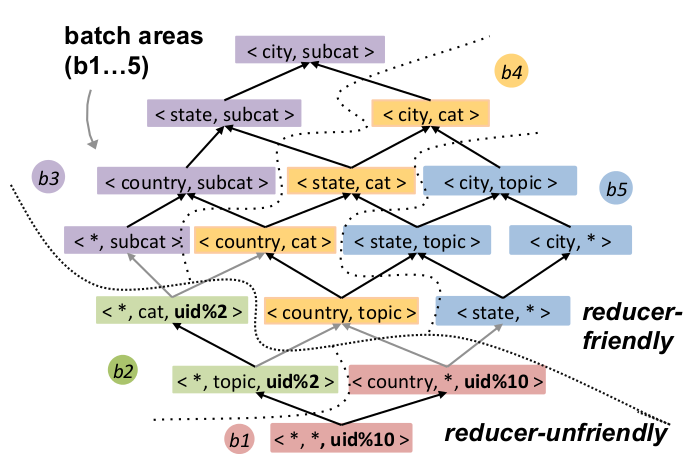
\includegraphics[width=3.5in]{picture/ch_datacube_mr/batch_area} 
\caption{Batch Area}\label{batch_area} 
\end{figure}

对于同一个 batch 内的 group 要如何计算有很多方法,论文使用的是BUC,(bottom up cubing algorithm)。但这种方法需要对数据扫描多次,而 Mapreduce 的 reducer 中提供的迭代器仅能对数据扫描一次,若要对数据进行多次扫描,则需要载入内存中。并且 BUC 这种方法也未充分利用 Mapreduce 框架的特性,例如排序功能。因此这里可以考虑替换其他的方法。同时,论文中只给出了batch 划分的规则,提到可用枚举、局部贪心或者模拟退火的方式找出合乎规则的 batch,并没有给出具体的方法,而模拟退火这样的计算方法又稍微复杂。因此这里可以考虑提出简单而有效的划分方法。


\section{贡献与不足}

MR-Cube \cite{nandi2011distributed} 这篇论文对使用 Naive 算法计算整体性度量函数的数据立方中存在的问题提出了一些非常有效的改善方法,论文的主要贡献包括:

\begin{enumerate}
\item 提出了对整体性度量划分的方法。
\item 提出了如何判断 group 是否需要划分,以及其划分的方法。
\item 提出了将多个 group 合并一起计算的 batch area 的概念。
\end{enumerate}

但是以上的方法也存在一些问题。

\begin{enumerate}
\item 论文中通过 region 内的一个大 group 将一个 region 内的所有 group 都贴上 reducer-unfriendly 的标签,导致 region 内所有的 group 都要划分。有些情况下可能一个 region 就只有一个大 group,而其他的 group 都很小,这样就导致了不必要的划分和加重后续的合并操作。
\item 论文中使用求余(\%)方法对数据进行划分,求余是一种哈希方法,但是这种哈希方法在一些情况下,可能会导致划分的不均匀。
\item Batch area 内的计算,也就是多个 group 之间的计算,论文里使用的 BUC 的方法,虽然这种方法很合适有阈值限定的情况(例如 HAVING),但是它需要对数据进行多次扫描,并且没有很好地利用 Mapreduce 本身的一些优势,例如排序。
\item 论文中只给出了 batch area 的规则,并没有提供简单且能满足规则的划分方法。
\end{enumerate}

针对以上4点,本论文提出了 TSP-Cube,将Tera-Sort、Pipesort 与数据立方的计算相结合,从而改进对 MR-Cube 的不足。






\chapter{TeraSort与数据立方的结合}

TeraSort \cite{o2008terabyte} 最初的提出是用于在 MapReduce 中对全局数据的排序。\cite{tao2013minimal} 提出了 TeraSort 最佳的采样比例,并证明了该比例的合理性。该论文同时将 TeraSort 与 GroupBy 结合,提高在倾斜数据集况下 GroupBy 的计算效率。由于 GroupBy 是数据立方的子操作,因此受到这篇论文的启发,考虑将TeraSort与数据立方相结合。

\section{TeraSort}

TeraSort最初用于在 MapReduce 中对全局数据的排序。虽然 MapReduce 输出的最终结果是有序的,但仅是每个 reducer 输出的数据是有序的,而 reducer 之间的数据是无序的。图\ref{tera_sort}为不使用 TeraSort 与使用 TeraSort 的情况下对原数据使用 MapReduce 排序的结果。图中每个矩形内的数据表示 每个 reducer 的输出。对于不使用 TeraSort 的MapReduce,每个 reducer 输出的数据都是有序的,但是reducer 之间的数据是无序的。而对于使用 TeraSort 的 MapReduce,不仅仅是每个 reducer 内的数据是有序的,reducer 之间的数据也是有序的。

\begin{figure}[ht] 
\centering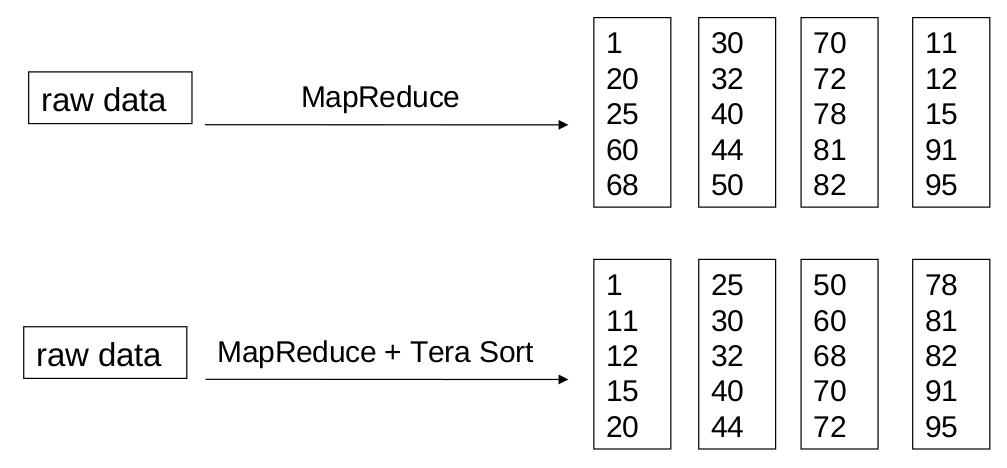
\includegraphics[width=4.5in]{picture/ch_terasort_mr/tera_sort} 
\caption{Tera Sort}\label{tera_sort} 
\end{figure}

TeraSort 能令全局有序的重要关键是,控制落到每个 reducer 上的数据的数据范围。也就是规定某一个范围内的数据必须落在指定的 reducer 上,而不是使用 MapReduce 本身的哈希函数将这些数据随机分发到各个 reducer 上。但如何确定这些范围值与 reducer 之间的关系呢,尤其是对原数据的数据特征并没有太多了解的情况下。这里使用采样的方法。

对原数据进行一定比例的采样,这个最佳比例 \cite{tao2013minimal} 已给出证明。接着将采样的数据都发到同q一个 reducer 上。根据 MapReduce 的特性,同一个 reducer 内的数据会被排序。若采样的样本大小为 s,reducer 的数量为 t。那么要从采样序列中选取 t-1 个点作为分界点,这些分界点是限定落入 reducer 中的数据的数据范围。对于第 i 个分界点选取的方法是,选取采样序列中的第 $i\times \left \lceil \frac{s}{t} \right \rceil$ 作为第 i 个分界点。图 \ref{tera_sort_mr1} 为  TeraSort 采样以及选取分界点的过程。图中假设 reducer 数据量为4,因此选取的分界点数量为3,红色的数字表示其被选为分界点。图中选取了3个分界点,分别为25、50、78,这就给出了4个 reducer 接收的数据范围,分别是$\left[- \infty, 25 \right], \left(25, 50 \right], \left(50, 78 \right], \left(78, +\infty \right]$。

\begin{figure}[!htb] 
\centering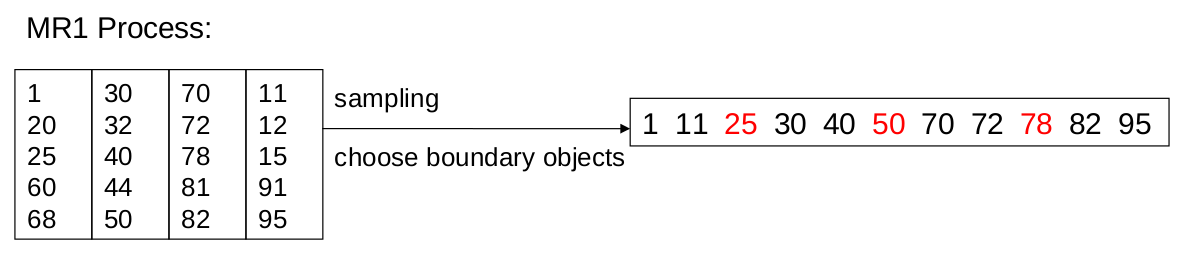
\includegraphics[width=6in]{picture/ch_terasort_mr/tera_sort_mr1} 
\caption{Tera Sort 采样与选取分界点}\label{tera_sort_mr1} 
\end{figure}

以上是第一轮 MapReduce,主要工作是采样以及选取分界点。这些分界点的作用是规定数据必须根据不同的范围落入既定的 reducer 上。在第二轮的 MapReduce 中,对于 Mapper 输出的每一条键值对,根据 key 的值,可使用二分查找等方法(Hadoop中使用Trie树)确定每一条键值对需要分发到的 reducer。最终 MapReduce 的结果就能全局有序。因此这里需要两轮 MapReduce。

\section{TeraSort与GroupBy}

\cite{tao2013minimal} 中将 TeraSort 与 GroupBy结合,能很好地解决倾斜数据集中由于各个 reducer 接收到的要计算的数据量差别过大,导致部分 reducer 运行时间过长的情况。

首先阐述使用 MapReduce 计算 GroupBy 的一般方法(称为Base GroupBy)。其实这个方法与 使用 MapReduce 计算数据立方的 Naive 方法类似。在 数据立方中,mapper的输出是每一条记录与所有 region 的映射。而在 GroupBy 中,仅需要与一个 region,即 GroupBy 的 region 映射即可。例如记录 e1=[a0, b0, c0, d0, m0],其中a0, b0, c0, d0对应的是维属性,m0 对应的是度量属性。当前操作是 GroupBy(B),那么对于这条记录输出的 key 为 b0,value 为 m0。具有相同的 key 值的数据会被分发到同一个 reducer 上计算,也就是具有相同 group\_value 的数据会被分发到同一个 reducer 上计算。如果数据集是倾斜的,也就是这个 region 内有一些特别大的 group,这将导致有一些 reducer 分发到大量的数据,而一些 reducer 分发到较少量的数据,导致最终计算效率的下降。

将 TeraSort 与 GroupBy结合,目的是将 region 内较大的 group 进行划分,从而将一个 group 分发到多个 reducer 上进行计算。而 TeraSort 的采样以及分界点的选择恰好能对大的 group 进行划分在。论文中以度量函数 SUM 作为例子,采样的数据是维属性与记录编号组成的组合键。也就是采样的key是[group\_value, tuple\_id]这样的组合键。之后的操作与 TeraSort 类似,将采样的数据发到一个 reducer 上,采样的数据会被排序,然后根据 reducer 的数量选取分界点。由于这里的key是复合键,因此在 group\_value 相同的情况下会比较 tuple\_id。也正因为这个tuple\_id,较大的 group 才能被划分。

图 \ref{base_groupby} 是使用 TeraSort 方法对采样的数据进行划分的示例。图中每个矩阵表示一个 group,矩阵越大,表示采样数据中具有相同 group\_value 的样本越多。红色的线表示分界点。分界点之间的间距是基本相同的,因此对于较大的 group 很有可能从中选取一个或多个分界点,正好将 group 进行了划分。若采样的key中只有 group\_value,而没有 tuple\_id,那么对于一个大 group,就算从中选择了多个分界点,但分界点的值都是相同的,这样的分界点就没有意义了。

图中每个分块都标有数字,各个分界点之间的分块会分派到同一个 reducer 上计算,但由于 group\_value 的不同,即使这些分块分到同一个 reducer 上,也会多次调用 reduce 函数。只有同一个 reducer 中具有相同 group\_value 的数据才会放在同一个 reduce 函数中进行计算。

\begin{figure}[!ht] 
\centering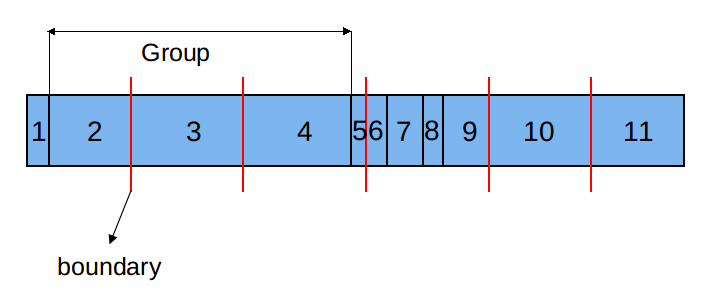
\includegraphics[width=4in]{picture/ch_terasort_mr/ts_groupby} 
\caption{使用TeraSort划分GroupBy的计算}\label{ts_groupby} 
\end{figure}

以上的采样以及选取分界点是第一轮的 MapReduce。第二轮的 MapReduce 与上面提到的计算 GroupBy 的一般方法类似,只是 key 的输出不仅仅是 group\_value,还需要tuple\_id。这样才能通过与分界点的比较确定数据要分发到某个确定的 reducer 上。使用 TeraSort 计算 GroupBy 还需要第三轮的 MapReduce,因为在上一轮的计算中,大的 group 被划分了,因此第三轮的 MapReduce 是对被划分的 group 进行合并。

\section{TeraSort与数据立方}

由于 GroupBy 是数据立方的一个子操作,受到 TeraSort 与 GroupBy 结合的启发,自然地引申到了 TeraSort 与数据立方的结合,并且发现这样的结合能解决上一章中提到的 MR-Cube 存在的一些问题。为了方便,以下将 TeraSort 与数据立方结合的方法称为 TS-Cube。

\subsection{数据采样与划分}

无论是 MR-Cube 还是 TS-Cube 都要解决一个问题,那就是大 group 的划分问题。在 MR-Cube 中是通过采样,然后根据采样数据中 group 的大小确定 region 是否为 reducer-unfriendly region。对于 reducer-unfriendly 的region,region 内的 group 都需要进行划分。MR-Cube 使用对某个属性值求余的方法对数据进行划分。对于 TS-Cube,运用 TeraSort 的思想,则同样需要采样,然后对采样数据排序,选取分界点。在 GroupBy 的场景下,采样的 key 是 [group\_value, tuple\_id] 这样的复合键,在数据立方的计算中,由于计算的不仅仅是一个 region,因此采样的 key 更为复杂。并且\cite{tao2013minimal} 中讨论的度量函数仅是 SUM,而这里还需要考虑到整体性度量函数。

首先考虑采样的 key 值。采样的 key 值关系到分界点的选取以及第二轮 MapReduce 计算时 reducer 中数据的均匀性。因为数据立方的计算涉及到多个 region,因此复合键中要加入与 region 有关的信息,这里选择加入 region\_id。将各个 region 按照字符串顺序排序,然后对它们编号,即可得到 region\_id。这样使用[region\_id, group\_value] 复合键即可表示一个指定 region 内指定的 group。但仅用这两个值对于大的group是无法划分的。因为若两个分界点落在同一个region的同一个group内,这两个分界点的值也是相同的,因此这里需要加入更多的信息。

在第二章准备知识中一共提到三种度量函数,这里可将这三种度量函数分为两类,一类是非整体性度量,另一类是整体性度量。以下分别阐述这两种不同的度量在采样时 key 值的构成。

对于非整体性度量,由于数据划分不受限制,因此数据不需要按照某个特定的属性进行划分。所以这里可以与选择 tuple\_id 作为 key 值的一部分。并且 tuple\_id 一般是数据的主键,主键是无重复的。这种情况下,一个 group 内若有多个分界点,分界点的值也是不同的。因此,对于非整体性度量函数,采样时的key为 [region\_id, group\_value, tuple\_id]。

而对于整体性度量,随意的数据划分对它的计算很可能是无任何帮助的。在这里,可使用 \cite{nandi2011distributed} 提出的部分线性度量(Partially Algebraic Measure)。也就是根据不同的整体性度量函数按照某个特定的属性值进行划分,而这个属性值在多数情况下都是度量属性值。因此,对于整体性度量函数,采样时的key为 [region\_id, group\_value, measure\_value]。这种情况下,即使一个 group 内有多个分界点,因为度量值的不同,分界点的值也不同。

同时,这样的划分对于计算也是有一定帮助的。例如 COUNT(DISTINCT(uid)),uid 为度量值,那么采样的key为 [region\_id, group\_value, uid]。因此相同的 uid 必定会划分到同一个分块内,因此对于每个分块仍然可以计算 COUNT(DISTINCT(uid)),然后对每个分块的结果做累加即可。图\ref{tscube_picture} 为 TS-Cube 的采样与分界点的选取。每一个矩阵表示一个 group,相同颜色的矩阵表示同一个 region 内的 group。红色的直线表示分界点。

\begin{figure}[!htb] 
\centering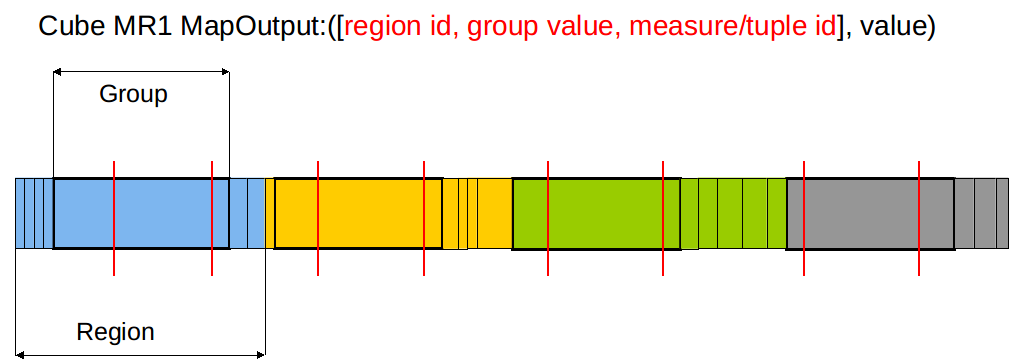
\includegraphics[width=6in]{picture/ch_terasort_mr/tscube_picture} 
\caption{TS-Cube的采样与分界点的选取}\label{tscube_picture} 
\end{figure}

根据以上的方法所选取的分界点即规定了每个 reducer 所要处理的数据范围。group 越大,采样中所占的比例也越大,那么分界点越容易落在其上。因此能达到大group被划分的目的。而对于分界点数量,若有 t 个reducer,则至少要选取 t-1 个分界点。但其实可以选择更多分界点,只要保持是 (t-1) 的倍数关系即可。但这个倍数到底如何选择,目前仍未有一个较好的结论。

\subsection{数据立方的计算}

以上的采样与分界点的选取是第一轮的 MapReduce,也即是对数据的划分。第二轮进行的 MapReduce 是对数据立方的计算。这里先不考虑将多个 group 的数据放在同一个 reduce 函数里计算的情况(即MR-Cube 中提出的 Batch Area),仍采用 Naive 的方法,映射所有的region。TS-Cube 与 Batch Area 的结合将在下一节中阐述。

根据使用 TeraSort 对数据进行全局排序以及计算 GroupBy 可看出来,第二轮的 MapReduce 中 mapper 输出的 key 一般与采样的 mapper 所输出的 key 是一致的。因为第一轮 mapper 输出的key中的若干个会被选为分界点,第二轮mapper的输出必须与第一轮保持一致,才可以与分界点进行比较,从而决定键值对落到哪个 reducer 上。决定键值对被分派到哪个 reducer 是在 MapReduce 的 partition 阶段。因此 mapper 输出的 key 与分界点的比较也正是在 partition 阶段。

而在 reduce 阶段,同一个 reducer 内的数据,若具有相同 region\_id 和 group\_value 则会在同一个 reduce 函数内进行计算。此处 reducer 的计算与 Naive 是一样的,因此不再详细说明。


这里需要为 MapReduce 的机制进行一些说明。在默认的 MapReduce 中,只有相同的 key 值的数据才会放在同一个 reduce 函数中计算。而在 TS-Cube 第二轮 MapReduce 中 mapper 输出的 key 值为 [region\_id, group\_value, tuple\_id or measure\_id],是一个复合键。按照默认规定,必须这3个值都相同才能放在同一个 reduce 函数内计算。但其实MapReduce的框架为此提供了灵活的变化。用户可重载 GroupPartitioner 函数,此函数是定义在同一个 reducer 内,具有什么特征的数据会被放在同一个 reduce 函数中计算。由于TS-Cube 的特殊性,这里需要重载 GroupPartioner,规定只要 region\_id 和 group\_value 相同的数据即可放在同一个 reduce 函数内计算。

最后进行第三轮的 MapReduce,将被划分的数据进行合并。


\subsection{实现伪代码}




使用 TeraSort 这样的采样与数据的划分方式正好可以解决 MR-Cube 中 group 的划分问题。在 MR-Cube 中,只要一个 region 内有一个大 group,那么这个 region 内所有的 group 都要被划分。而在 TS-Cube内,分界点一般只会落在较大的 group 上,即使不落在较大的 group 上,也只会落在两个小的 group 之间。因为 group 越小,采样中出现的数量也越少,那么分界点落在这个小 group 上的概率也就非常小了。只有分界点落到的 group 才会被划分,这样 TS-Cube 一般只会划分大的 group。因此 TS-Cube 就可以避免了 MR-Cube 中出现的不必要的划分。

在 MR-Cube 中使用求余的方式对数据进行划分,在一些极端情况下,可能数据会有倾斜性,导致划分后的数据依然有倾斜性。例如使用 MR-Cube 的方法计算的划分因子的结果是2,也就是令某个属性值对2求余从而达到数据划分的效果,而需要划分的属性值若大部分都是奇数,这样将导致数据划分的失效。而使用 TS-Cube 的方法则可以避免这种情况。即使所有的度量属性值都是奇数,TS-Cube 依然可以较为均匀地划分数据。因为 TS-Cube 对数据的划分是基于数据出现的频率,数据出现频率越高,越容易被划分,也正好达到了大数据需要划分的目的。


\section{TS-Cube 与 Pipesort}



\subsection{PipeSort}



\subsection{TS-Cube 与 PipeSort 的结合}


\subsection{实现伪代码}



\section{TSP-Cube 与 MR-Cube的比较}










\chapter{实验}

实验中使用多种不同分布的数据集,比较多种在 MapReduce 框架下计算数据立方的方法,分别从运行时间、各个reducer处理的数据量、合并的数据量等角度进行比较。实验结果表明,没有任何一种方法是``万能”的,根据不同的度量函数、数据分布,不同的方法各有优势。对于代数度量函数,Naive的方法足以解决计算。而对于整体性度量函数,TSP-Cube相比MR-Cube,不仅仅在性能上有优势,同时还能处理更多不同的倾斜的数据分布,更具有通用性。

\section{实验环境}
实验的环境使用 Hadoop 1.0.4 所搭建的集群。节点数为7,每个节点的CPU为4核 Intel Xeon 2.4GHz,内存为24GB。每个节点的JVM分配的内存大小为6G。Reducer的数量为20。

\section{实验数据集与度量}

实验的数据集使用前两个章节提到的具有层次型的数据集,如图 \ref{dataset_table} 所示。表中共有 6 个维属性,分别是 country,state,city,topic,category,subcategory。其中\textless country, state, city\textgreater 是具有层次型的,同理\textless topic, category, subcategory\textgreater 也是具有层次型的。因此在 GroupBy 时,GroupBy(country, state, topic) 和 GroupBy(state, topic)是等价的。并且不会出现 GroupBy(country, city, topic) 这样的跨越层次的操作。该数据集对应的 lattice 如图 \ref{dataset_lattice} 所示。由于数据集具有层次型,因此lattice中region总数量为16。

\begin{figure}[!htb]
\centering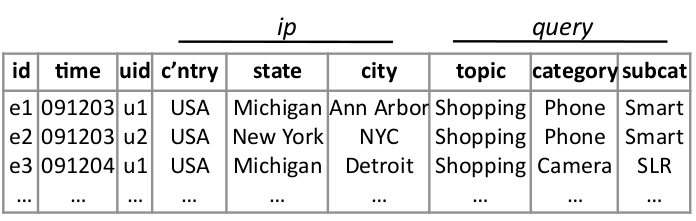
\includegraphics[width=3.5in]{picture/ch_datacube_mr/dataset_table} 
\caption{数据集的表结构}\label{dataset_table} 
\end{figure} 

\begin{figure}[!htb]
\centering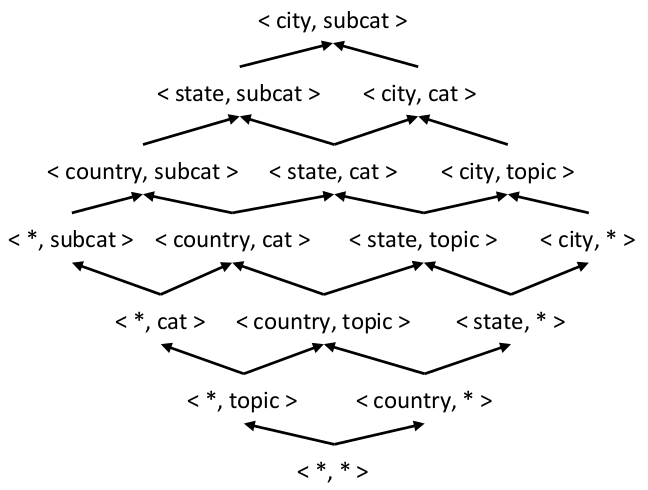
\includegraphics[width=3in]{picture/ch_datacube_mr/dataset_lattice} 
\caption{数据集的lattice}\label{dataset_lattice} 
\end{figure} 

对于该数据集,为了充分比较各种算法的效率与特性,实验中使用了3种不同的数据分布。分别如下:
\begin{itemize}

\item \textbf{D1 分布}

对于属性 country 的取值范围为 [1,3],且是均匀分布的。对于属性 topic 的取值范围为[1,10],且是均匀分布的。剩余的属性取值范围较大,如city取值范围为[1,4000],subcategory 取值范围为[1,20000],且都是均匀分布的。由于country和topic的取值范围较小,因此Region(country)和Region(topic)在数据量较大的数据集中均包含了大的group。

\item \textbf{D2A 分布}

为了出现数据分布更倾斜的情况,即每个region中都有reducer-unfriendly的group,因此该分布中的数据是2/8分的。这里的2/8分指的是该数据集中有80\%的记录,它们之间的6个维属性都是相同的,即它们都属于同一个group,剩下的20\%的数据的分布与 D1 相同。而对于非维属性,它们的取值则无此特性,属性 uid 是均匀分布的。

\item \textbf{D2B 分布}

D2B 的数据分布与 D2A 基本一致,但 uid 是倾斜分布的,若使用求余的方式对数据进行划分,则可能导致划分的不均匀。

\end{itemize}

这三种数据集都有不同程度的倾斜,D1的倾斜度没有D2的明显,并且D1数据集中仅有部分的region是reducer-unfriendly的,例如Region(country)、Region(topic)。而对于D2的数据集,在数据量较大时,每个region都会是reducer-unfriendly的region。对于以上三种分布,属性 uid 的取值范围均为$[1,{10}^{6}]$。由于uid取值范围较大,因此MapReduce的combiner无法充分发挥作用。

实验中分别对代数度量与整体性度量进行比较,代数度量选择 COUNT(*),计算每个group内记录的数量; 整体性度量选择 COUNT(DISTINCT(uid)),计算每个group内不同的uid数量。

数据集中记录的数量分别为${10}^{6}$、${10}^{7}$、${10}^{8}$、${10}^{9}$。对于${10}^{9}$的数据集,大小约为45G。


\section{比较算法}

TSP-Cube 除了与 Naive 和 MR-Cube 的方法比较外,还将与 Naive-Pipesort 与 TopDownCube \cite{lee2012efficient} 进行比较。

Naive-Pipesort 是不对group进行任何划分,只将多个group放在同一个reduce函数内计算,并且使用与TSP-Cube一致的计算方法——Pipesort 计算同一个reduce函数内的多个group。将TSP-Cube与这个方法比较,是为了查看当数据倾斜时,reduce是否会出现严重的负载不均衡,并且查看数据划分是否能提升计算效率。

TopDownCube,是将 Pipesort 与 MapReduce 结合的一种方法。Pipsort最根本的思想是对``数据”不断地排序,这个``数据”可能是原数据,也可能是已经计算好GroupBy的数据。TopDownCube沿用了\cite{agarwal1996computation} 中构造pipe树的方法,并且使用 MapReduce 对每个pipeline中的数据都按照起始 region 的属性顺序进行排序。这个方法的缺点是需要执行多次MapReduce,因为该方法会对于每个 pipeline都执行一次 MapReduce,将数据按照起始region的属性顺序排序。排序后它可以将多个 region 放在同一个 reducer 上计算,并且由于不是所有排序都基于原数据,因此产生的中间数据比 Naive-Pipesort要少。但这种方法并没有考虑整体性度量函数,因此该方法更适合代数度量函数的计算。

实验代码GitHub地址:\url{https://github.com/abcdmyz/MapReduceDataCube}

\section{实验结果}

对以上算法的比较主要包括,在不同的数据分布以及数据大小下,算法的运行时间, 各个reducer输入的记录数。通过算法的运行时间比较各个算法的效率,通过各个 reducer 输入的记录数查看数据划分对各个reducer 之间的负载均衡影响。最后还比较了 MR-Cube 与 TSP-Cube 在第二次MapReduce后,即数据立方计算后,需要合并的数据量,以及 TSP-Cube 3次MapReduce各占的比例。

以下分别从不同类型的度量函数来分析实验结果。

\subsection{DISTINCT 度量}


图\ref{d1_distinct_time}、 \ref{d2a_distinct_time}、 \ref{d2b_distinct_time} 分别为在 D1, D2A, D2B 三种不同的分布下,5种方法计算COUNT(DISTINCT(uid))度量函数的运行时间。图中的横轴为数据大小,图中的纵轴为运行时间,单位为分钟。从图中可看出,当数据量较小时,5种方法之间的差距并不大,当数据量到达${10}^{9}$时,各种方法之间才有较为明显的差距。图\ref{d1_distinct_input}、图\ref{d2a_distinct_input}、图\ref{d2b_distinct_input} 分别为数据集大小为${10}^{9}$时,各种方法中各个reducer输入的记录数。从这个记录数查看各个reducer之间的负载差距。以下分别分析各种方法的运行时间以及reducer的负载。

\begin{itemize}

\item \textbf{Naive, Naive-Pipesort}

Naive方法 无论在任何一种分布下所花费的时间都是最多的。在D1的数据分布下,Naive-Pipesort的方法的运行时间是最短的,但与MR-Cube和TSP-Cube相比,优势并不大。在D2的分布下,Naive-Pipesort的性能则大打折扣。这是因为对于极端倾斜的数据分布,就算在Naive的基础上加上了PipeSort,但由于D2中的一些group的大小差距非常大(D2是2/8分的分布),而这些大group并没有进行划分,导致 reducer之间的负载极度不均衡,最终仍然使性能下降。由于D2的倾斜性比D1明显,因此Naive-Pipesort的缺点在D2中更能体现。从图\ref{d2a_distinct_input}和图\ref{d2b_distinct_input} 可看出 Naive-Pipesort 的方法各个reducer输入的数据量有较大的差距,尤其有3个reducer输入的数据量特别大,导致了整体的执行时间变长。

\item \textbf{TopDownCube}

对于 TopDownCube的方法,在D1中仅比Naive的方法好,这是因为它要进行多次的MapReduce对数据进行排序,但uid的取值范围较大,无法大量压缩,中间数据仅减少了小部分,多次``低效”的排序导致它需要较长的运行时间。而在D2A分布中,它比Naive-Pipesort的方法有优势。因为 D2A 的数据比 D1 更倾斜,对于Naive-Pipesort而言,其负载不均衡的情况比 TopDownCube更严重。因为TopDown通过对数据多次排序,减少了部分的中间数据,尽管减少的量并不大,但是与Naive-Pipesort相比,能降低负载不均衡的严重性,因此TopDownCube 与 Naive-Pipesort 相比有一定的优势。

但与TSP-Cube相比,在任何一种数据分布中,运行时间都比TSP-Cube的要长,这也因为数据倾斜导致的。因为TopDown没有对数据进行划分,reducer之间的负载差距依然存在,即使它使用多轮MapReduce减少中间数据。从图\ref{d1_distinct_input}、图\ref{d2a_distinct_input}可看出TopDownCube中各个reducer之间有一定差距,而TPS-Cube的各个reducer之间是非常均匀的。总体而言,将TopDownCube的方法运用在计算整体性度量函数中,优势并不明显。

\item \textbf{MR-Cube, TSP-Cube}

TSP-Cube与MR-Cube相比,在三种分布下,TSP-Cube的运行时间都比MR-Cube少。在D1和D2A中,这种时间优势并不明显,差距并不大,但在D2B中,TSP-Cube的优势则较为明显地体现出来。对于D1,从图\ref{d1_distinct_input} 中可看出,MR-Cube的各个reducer之间要处理的数据量会有一定的差距,而TSP-Cube的各个reducer的数据量非常均匀,因此TSP-Cube比MR-Cube在时间上稍微有优势。

对于D2A,MR-Cube与TSP-Cube的时间差也不大,从图\ref{d2a_distinct_input}中可看出 MR-Cube 与 TSP-Cube 的各个reducer上的数据都是均匀的,导致两者细微的差距是第三轮MapReduce中要合并的数据量的差距。图\ref{d2a_distinct_interdata} 为 MR-Cube与TSP-Cube第三轮需要合并的数据量的比较。从图中可看出,MR-Cube相比TSP-Cube要合并更多的数据,因此需要更多的时间。对于D2B,因为D2B中的uid分布是不均匀的,这样MR-Cube中使用求余的方式对数据进行划分,可能导致划分后的数据依然不均匀。Reducer之间的负载差距则导致MR-Cube性能的下降。在图\ref{d2b_distinct_input}中,由于uid的倾斜性,导致MR-Cube的各个reducer分布不均匀,但TSP-Cube的各个reducer中的数据依然能够均匀分布。因此TSP-Cube比MR-Cube在性能上有较大的优势。

\end{itemize}

\begin{figure}[!ht]
\begin{tabular}{cc}

\begin{minipage}[t]{0.45\textwidth}
\centering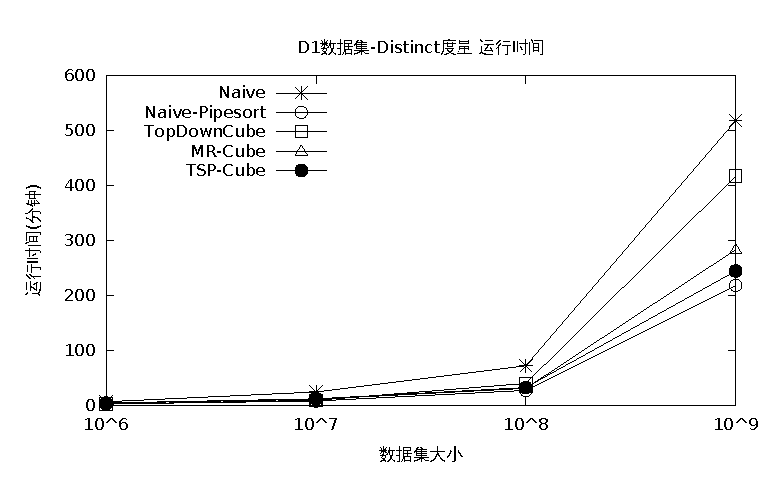
\includegraphics[width=2.7in]{picture/ch_experiment_gnuplot_eps/d1_distinct_time} 
\caption{D1-DISTINCT运行时间}\label{d1_distinct_time} 
\end{minipage}

\begin{minipage}[t]{0.55	\textwidth}
\centering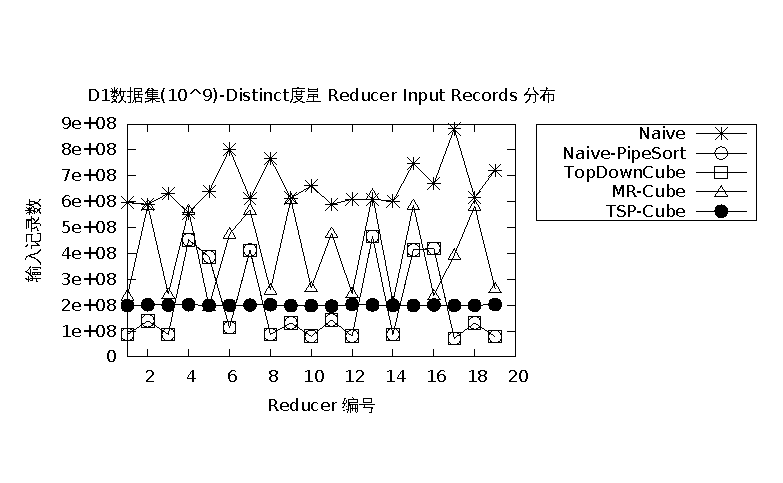
\includegraphics[width=3.2in]{picture/ch_experiment_gnuplot_eps/d1_distinct_input} 
\caption{D1-DISTINCT Reducer Input}\label{d1_distinct_input} 
\end{minipage}

\end{tabular}
\end{figure}



\begin{figure}[!ht]
\begin{tabular}{cc}

\begin{minipage}[t]{0.45\textwidth}
\centering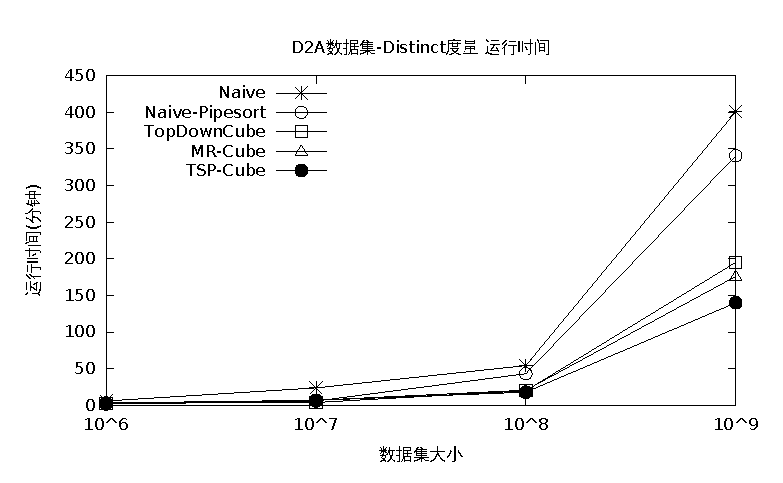
\includegraphics[width=2.7in]{picture/ch_experiment_gnuplot_eps/d2a_distinct_time} 
\caption{D2A-DISTINCT运行时间}\label{d2a_distinct_time} 
\end{minipage}

\begin{minipage}[t]{0.55\textwidth}
\centering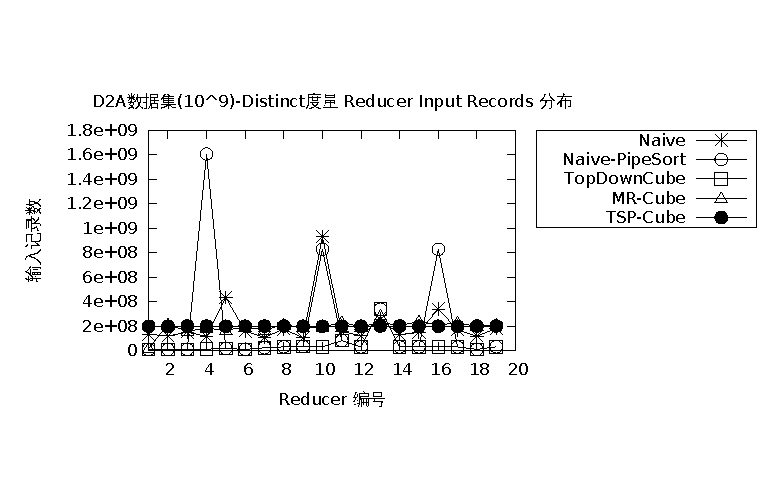
\includegraphics[width=3.2in]{picture/ch_experiment_gnuplot_eps/d2a_distinct_input} 
\caption{D2A-DISTINCT Reducer Input}\label{d2a_distinct_input} 
\end{minipage}

\end{tabular}
\end{figure}


\begin{figure}[!ht]
\begin{tabular}{cc}

\begin{minipage}[t]{0.45\textwidth}
\centering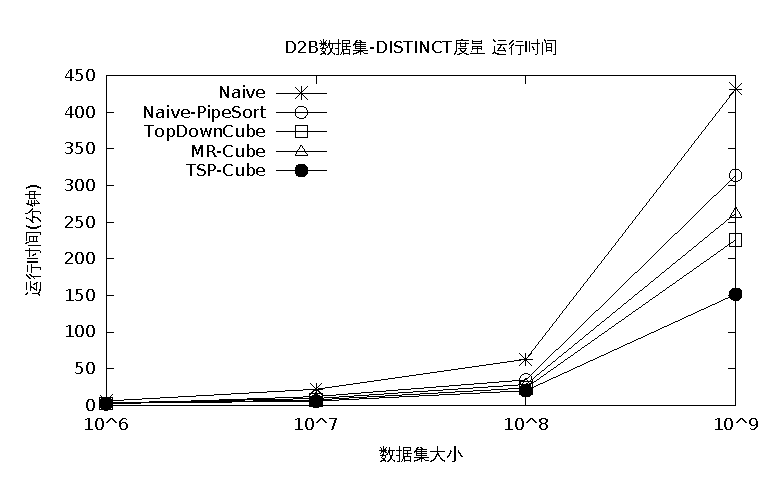
\includegraphics[width=2.7in]{picture/ch_experiment_gnuplot_eps/d2b_distinct_time} 
\caption{D2B-DISTINCT运行时间}\label{d2b_distinct_time} 
\end{minipage}

\begin{minipage}[t]{0.55\textwidth}
\centering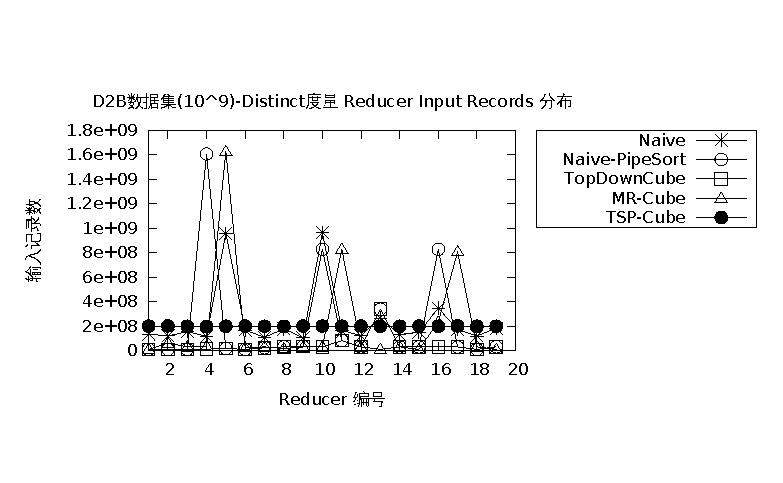
\includegraphics[width=3.2in]{picture/ch_experiment_gnuplot_eps/d2b_distinct_input} 
\caption{D2B-DISTINCT Reducer Input}\label{d2b_distinct_input} 
\end{minipage}

\end{tabular}
\end{figure}


除了比较运行时间与reducer的负载外,以下还将比较MR-Cube与TSP-Cube在不同分布下,在第三轮MapReduce时,需要合并的数据量,以及TSP-Cube的3次MapReduce分别占总时间的比例。在前面的章节提到,MR-Cube对group的划分方法在一些场景下会导致不必要的划分,从而加重了之后的合并操作,因此这里将两种方法需要合并的数据量进行比较,从而说明TSP-Cube需要进行合并的数据比MR-Cube更少。

图\ref{d1_distinct_interdata}和图\ref{d2a_distinct_interdata}分别为MR-Cube与TSP-Cube在D1和D2A数据分布下,需要合并的数据量。图\ref{d1_distinct_intertime}和图\ref{d2a_distinct_intertime}为合并时间。在D1中,由于数据倾斜性并不明显,因此两者需要合并的数据量差别不大,时间上差别也不大。但在D2A中,由于数据的倾斜性较明显,而MR-Cube会对数据产生不必要的划分,因此随着数据量增大,MR-Cube要合并的数据比TSP-Cube要多,合并时间更长。

图\ref{d1_distinct_mr123}和图\ref{d2a_distinct_mr123} 分别为TSP-Cube在D1和D2A数据分布,数据集大小为 ${10}^{9}$ 下,三次MapReduce占总体时间的比例。随着数据量增大,MR1和MR3所占的比例都会减少。因此花费一定代价对数据进行划分从而使数据分配均匀对总体性能的提升是有意义的。

从以上实验可看出,TSP-Cube相对于其他方法并不是``完美无缺”或者各方面``遥遥领先”的,它在一些数据分布下,跟大部分的方法相比,在性能上的优势并不明显。但在一些较为倾斜的数据分布下,它能表现出它性能的优势。TSP-Cube 无论在一般数据分布下,或者倾斜的数据分布下,均能对数据进行均匀的划分,令各个reducer上的数据负载均衡,从而提升计算性能。并且 TSP-Cube中的Pipesort方法简单且有效,能令数据立方计算过程中的中间数据大大减少,从而也提升了计算性能。因此由以上的实验得出,TSP-Cube 比 MR-Cube 更具有通用性,在一些更为倾斜的数据集下,有明显的优势。





\begin{figure}[!ht]
\begin{tabular}{cc}

\begin{minipage}[t]{0.5\textwidth}
\centering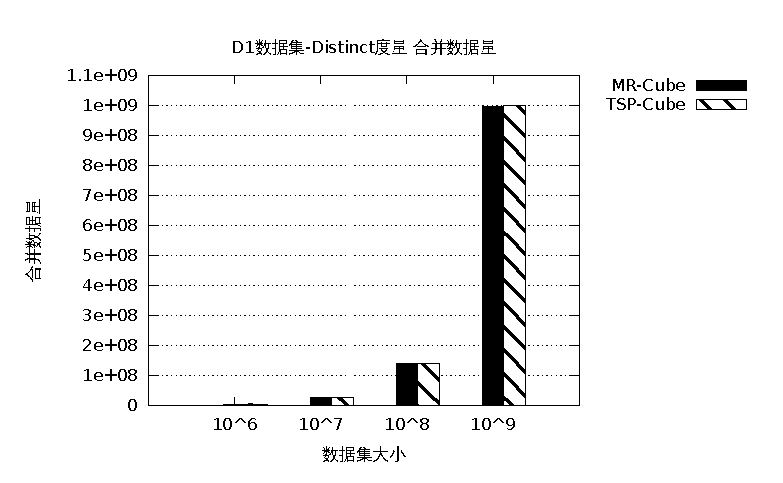
\includegraphics[width=3in]{picture/ch_experiment_gnuplot_eps/d1_distinct_interdata} 
\caption{D1-DISTINCT 合并数据量}\label{d1_distinct_interdata} 
\end{minipage}

\begin{minipage}[t]{0.5\textwidth}
\centering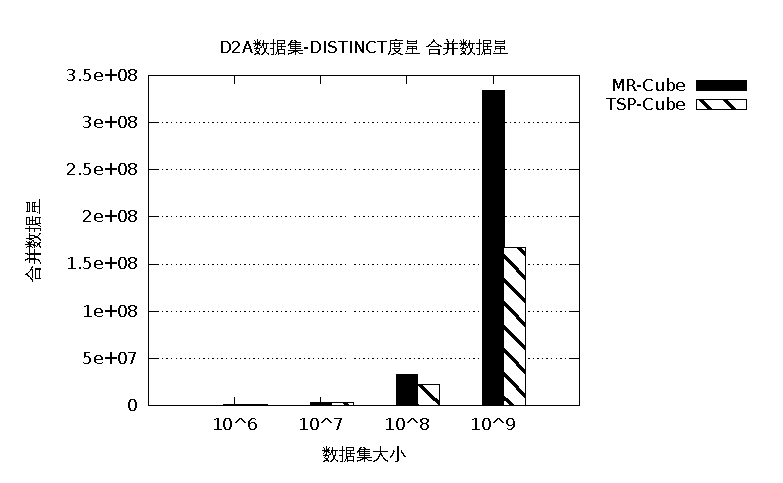
\includegraphics[width=3in]{picture/ch_experiment_gnuplot_eps/d2a_distinct_interdata} 
\caption{D2A-DISTINCT 合并数据量}\label{d2a_distinct_interdata} 
\end{minipage}

\end{tabular}
\end{figure}



\begin{figure}[!ht]
\begin{tabular}{cc}

\begin{minipage}[t]{0.5\textwidth}
\centering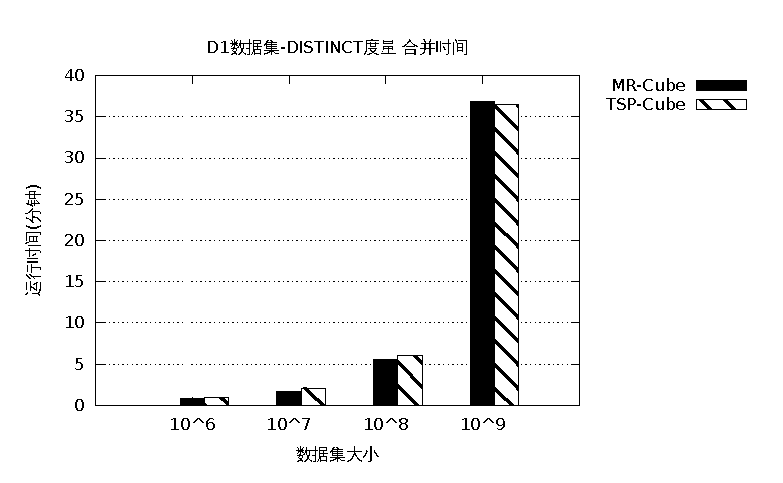
\includegraphics[width=3in]{picture/ch_experiment_gnuplot_eps/d1_distinct_intertime} 
\caption{D1-DISTINCT 合并数据时间}\label{d1_distinct_intertime} 
\end{minipage}

\begin{minipage}[t]{0.5\textwidth}
\centering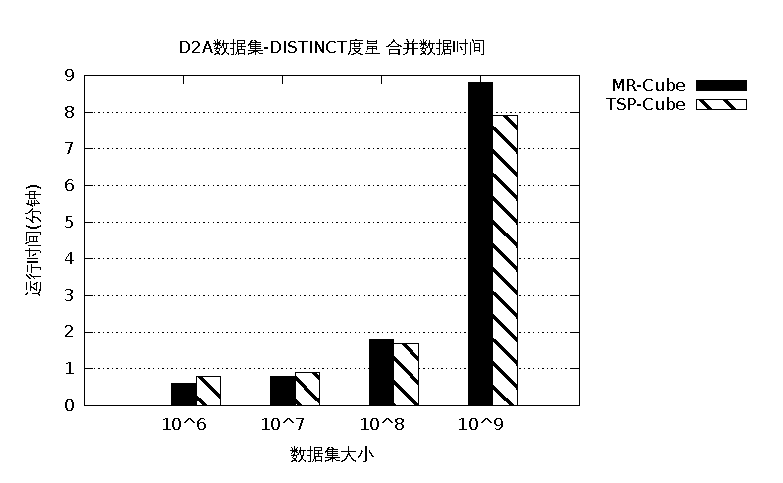
\includegraphics[width=3in]{picture/ch_experiment_gnuplot_eps/d2a_distinct_intertime} 
\caption{D2A-DISTINCT 合并数据时间}\label{d2a_distinct_intertime} 
\end{minipage}

\end{tabular}
\end{figure}





\begin{figure}[!ht]
\begin{tabular}{cc}

\begin{minipage}[t]{0.5\textwidth}
\centering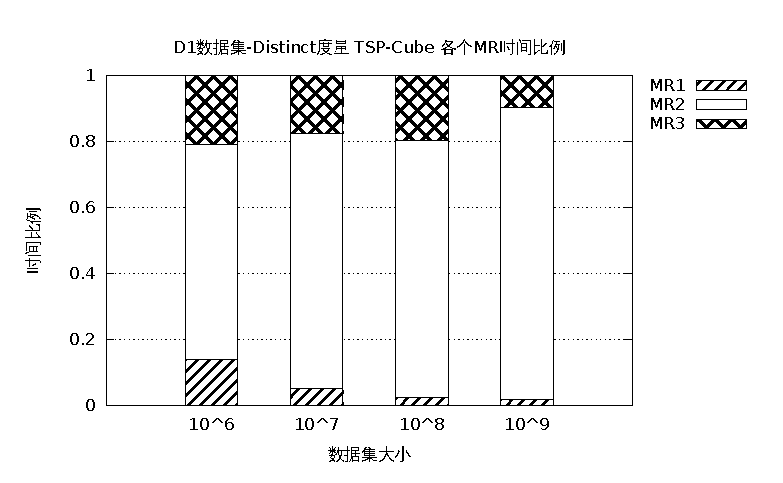
\includegraphics[width=3in]{picture/ch_experiment_gnuplot_eps/d1_distinct_mr123} 
\caption{D1-DISTINCT TSP-Cube 各个MR  运行时间比例}\label{d1_distinct_mr123} 
\end{minipage}

\begin{minipage}[t]{0.5\textwidth}
\centering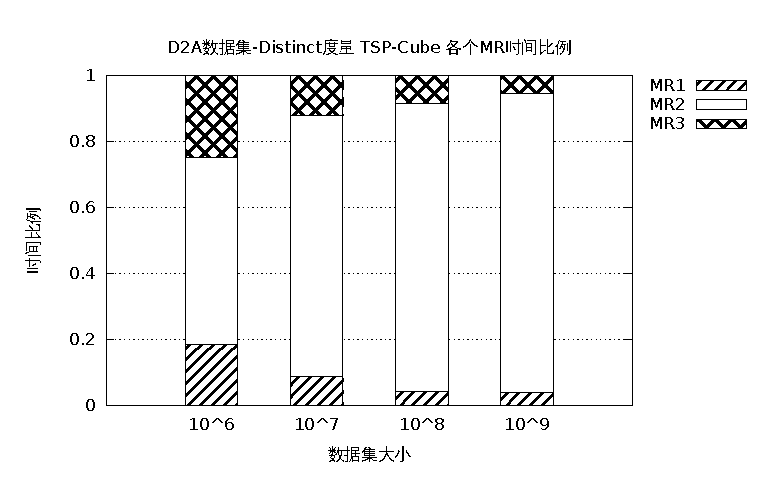
\includegraphics[width=3in]{picture/ch_experiment_gnuplot_eps/d2a_distinct_mr123} 
\caption{D2A-DISTINCT TSP-Cube 各个MR  运行时间比例	}\label{d2a_distinct_mr123} 
\end{minipage}

\end{tabular}
\end{figure}



\subsection{COUNT 度量}

在实验中加入代数度量函数进行对比,从而说明不同类型的度量函数应使用对应合适的方法,在分布式数据立方的计算中,并没有一种万能的方法可以适用于所有的度量函数和所有的场景。以下将5种方法计算COUNT的性能进行比较。图\ref{d1_count_time}、图\ref{d2a_count_time}分别为D1和D2A分布下,5种方法在不同数据大小下的运行时间。图\ref{d1_count_input}、图\ref{d2a_count_input}为不D1和D2A分布下,各个reducer输入的数据量。

从这些图中发现,在DISTINCT度量中性能表现最差的Naive,在COUNT度量中却是性能最好的,无论是在哪种数据分布下。在DISTINCT度量中,由于数据的倾斜性,Naive方法在reducer上数据的分布是非常不均匀的,但是在COUNT度量中,Naive方法在reducer上的数据分布却是非常均匀的,无论在哪种数据分布下。而TSP-Cube和MR-Cube对数据的划分反而导致数据的不均匀。

这个结果的出现与度量函数本身,还有MapReduce框架的特性有非常大的关系。COUNT是代数度量函数,因此数据可以随意划分,并且对于每个分块进行计算的中间结果都是一个整数,或者数据量是固定的。而MapReduce框架有一个非常重要的特性,Combiner。这个Combiner的作用在上一章节中也提到,它等同于本地的reducer。mapper产生的输出并不是直接发给相应的reducer,而是先在本地进行一次reduce计算,再通过网络传输发到reducer上。对于代数度量函数,一个group内的大量数据都可以变成一条数据发到reducer上,因此中间数据大大减少,并且mapper的数量是有限的,那么分发到一个reducer上一个group内的数据也是有限的。这样有限的数据必然不会导致各个reducer上数据的不均匀。

MR-Cube与TSP-Cube的提出,都是为了解决reducer上数据分配不均匀,数据量差别过大的问题,但在代数度量中,这个问题不存在,那么强行使用这两种方法只会带来更差的性能。从图中也可看出,Naive和TopDownCube在性能上比MR-Cube和TSP-Cube更有优势。

Naive-Pipesort的方法在计算COUNT度量时,性能不如Naive的方法,即使Naive-Pipesort方法的中间数据变少了,但性能反而比Naive的差。这是因为Pipesort要求对数据进行排序。MapReduce默认会对key进行排序,但是对于value,若用户不重载相关函数,value是不会排序的。而Pipesort是需要对value进行排序,这里需要花费一定的时间。因此即使Naive的中间数据比Naive-Pipesort多,但因为Naive不需要对value进行排序,因此在性能上能比Naive-Pipesort的更有优势。

\begin{figure}[!ht]
\begin{tabular}{cc}

\begin{minipage}[t]{0.4\textwidth}
\centering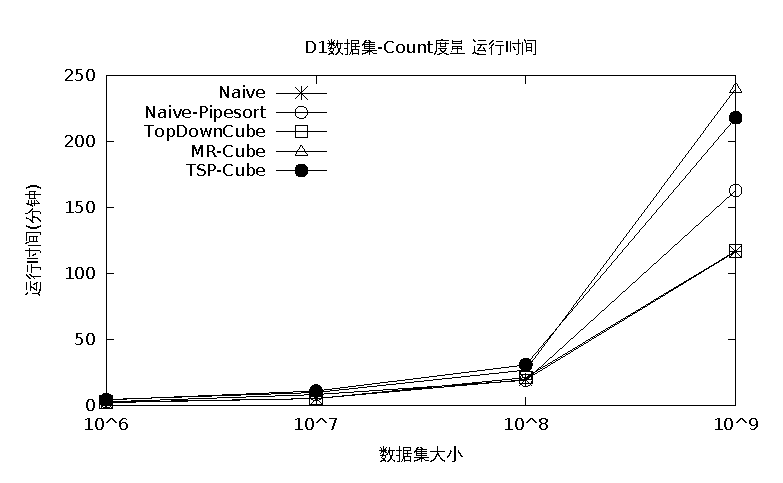
\includegraphics[width=2.7in]{picture/ch_experiment_gnuplot_eps/d1_count_time} 
\caption{D1-COUNT 运行时间}\label{d1_count_time} 
\end{minipage}

\begin{minipage}[t]{0.6\textwidth}
\centering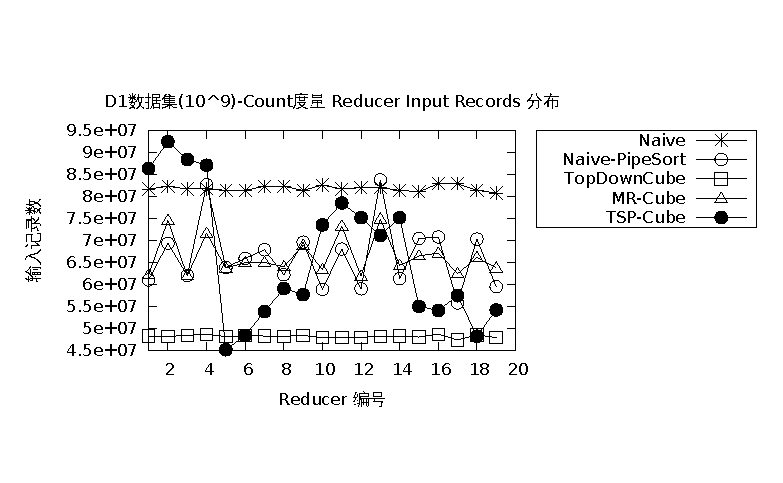
\includegraphics[width=3in]{picture/ch_experiment_gnuplot_eps/d1_count_input} 
\caption{D1-COUNT Reducer Input}\label{d1_count_input} 
\end{minipage}

\end{tabular}
\end{figure}


\begin{figure}[!ht]
\begin{tabular}{cc}

\begin{minipage}[t]{0.4\textwidth}
\centering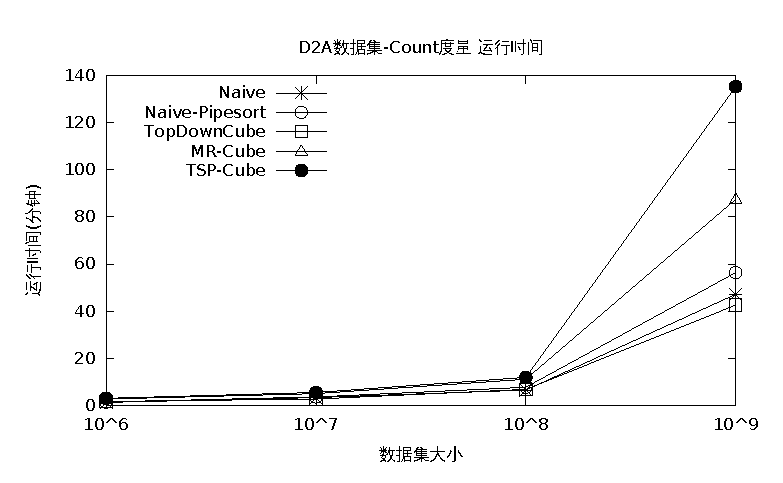
\includegraphics[width=2.7in]{picture/ch_experiment_gnuplot_eps/d2a_count_time} 
\caption{D2A-COUNT 运行时间}\label{d2a_count_time} 
\end{minipage}

\begin{minipage}[t]{0.6\textwidth}
\centering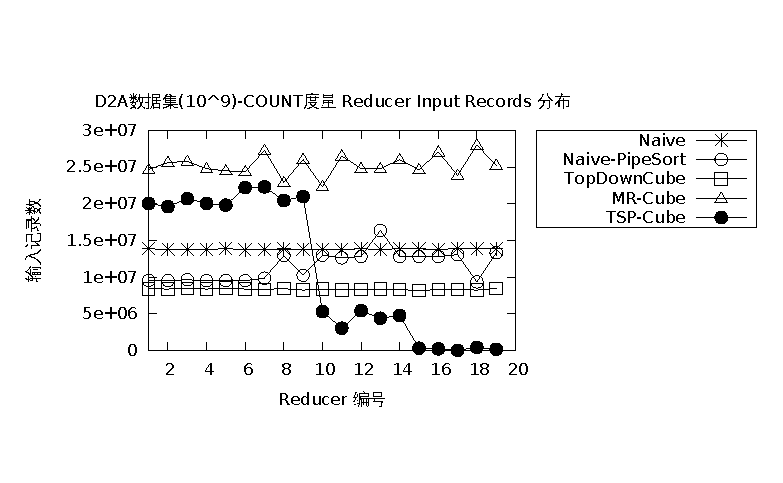
\includegraphics[width=3in]{picture/ch_experiment_gnuplot_eps/d2a_count_input} 
\caption{D2A-COUNT Reducer Input}\label{d2a_count_input} 
\end{minipage}

\end{tabular}
\end{figure}

\section{实验结论}

根据以上的实验,可得知不同的度量函数使用不同的方法会有不同的结果,目前没有一种方法能对于所有的数据分布、所有的度量都适用。在对一种方法进行评估时,需要考虑到它使用的场景(包括度量函数、数据分布等),还需要结合它所基于的框架的特性,来综合评估这种方法。Naive的方法即使简单,也并不是在所有情况下都效率低下,结合框架的特性反而能让它发挥优势。而相对复杂的TSP-Cube方法,则着重于解决一些Naive解决不了的更为极端的情况。

对于代数度量,使用Naive的方法已经足够了。Naive方法实现简单,并且在代数度量中,并不会出现reducer负载不均衡的情况。而对于整体性度量,TSP-Cube与多种算法相比,无论在一般分布或是倾斜分布下,性能都是最好的,尤其在极端倾斜的分布下,其性能优势更为明显。在负载均衡方面,即使在极端倾斜的分布下,TSP-Cube 依然能均匀地划分数据,这也是与其他算法相比最大的优势。由于TSP-Cube 在不同的场景不同的数据分布下,均能保持性能优势,比其他方法更具有通用性,因此建议对于整体性度量函数,使用TSP-Cube的方法。




\chapter{总结与展望}

数据立方是 OLAP 领域内一项关键技术,在现实应用中,数据立方的高效计算是实例化数据立方的关键。数据立方的高效计算可大幅度提高 OLAP 对查询的响应时间。分布式计算随着数据量爆炸式地增长,被越来越广泛地使用。因此将数据立方的计算与分布式结合是必然的趋势。数据立方的计算效率不仅仅与数据量有关,还与度量函数、数据分布等因素有关,因此数据立方的计算并不是简单地能用一种方法解决。尤其当它与分布式框架MapReduce结合时,可能带来更多的问题。

在数据立方的计算中,度量函数主要划分为两类,代数度量与整体性度量。对于代数度量函数,数据立方的计算相对更为简单,由于数据的可划分性与中间结果的确定性,它与MapReduce能很好地结合。但对于整体性度量函数,问题就变得复杂了。尤其当它与MapReduce结合时,由于数据的不可划分,在倾斜的数据集下,直接使用代数度量函数的方法来计算整体性度量函数,会给MapReduce带来负载不均衡的问题。MR-Cube 的提出正是解决在倾斜数据集下整体性度量函数的计算问题。它通过采样的方式确定数据集中是否有大group,从而对该region内所有的group进行划分,减少MapReduce负载不均衡的问题。同时它还提出了 BatchArea 的概念,将多个 group 放在同一个 reduce 函数内计算,减少中间数据的产生。

MR-Cube 虽然实现了数据立方与 MapReduce 的高效结合,但其仍存在缺陷,尤其是在极端倾斜的数据集下,会产生许多不必要的数据划分,从而加重之后的合并操作,而它对数据划分的方法也很可能退化失效。同时它对 batch 的划分只给出了一些建议遵循的规则,并没有给出具体的简单有效的划分方法。而且MR-Cube使用的BUC算法对batch内的group进行计算,并未能与MapReduce有非常好的结合。

针对以上不足,本文提出了一种TSP-Cube的计算方法。TSP-Cube 对 MR-Cube的改进主要分为两个方面。一个方面是改进了MR-Cube对数据的划分,借鉴TeraSort的思想对数据进行划分,可避免不必要的数据划分,减轻之后的合并操作。并且即使在极端倾斜的数据分布下,也能对数据进行均匀的划分,比MR-Cube对数据的划分更有通用性。另一方面,利用MapReduce的特性,提出使用 Pipesort 替换 BUC 计算 batch 内多个 group 的聚合。对 pipeline的形成方案 提出了更为直接简单并且有效的生成方法,尤其针对层次型的数据集和Pipesort的特点,给出了均匀且有效的生成 pipeline 的方法。

论文通过实验说明在不同的度量函数,不同的数据分布下,多种方法的差异,从而说明没有一种方法是可以解决所有的问题。通过实验结果可得出,对于代数度量函数,由于MapReduce框架的特性,使用Naive的方法足以应对计算。但当处理整体性度量函数的计算,尤其当数据具有倾斜性时,TSP-Cube比MR-Cube更具有通用性,可解决一般倾斜至极端倾斜的情况。

在未来的工作中,数据立方仍有许多需要探索的地方。一方面,整体性度量是更为复杂的度量,并且可能有嵌套的情况,这令数据划分变得更为复杂,因此需要研究总结出对数据划分更为通用的方法。另一方面,随着维度数量的增加,数据立方的大小呈指数型增长,因此部分数据立方的计算在这种情况下更有研究价值。甚至可以考虑使用采样,通过概率统计等方法估算数据立方的结果,这是一种为了实时性而牺牲精度的方法。最后,MapReduce只是分布式框架中的一种,之后的研究可以考虑是否有其他分布式框架更适合与数据立方的计算相结合。










本研究很有意义啊。

%\bibliographystyle{unsrt}
\bibliographystyle{sysuthesis}
\bibliography{main,reference}

%\appendix
%

\chapter{这是附录}


\section{附录是什么}
\Verbatiminput{}
附录是正文主体的补充。
下列内容可以作为附录:
\begin{enumerate}
\item 攻读学位期间发表的(含已录用,并有录用通知书的)与学位论文相关的
	学术论文目录
\item 由于篇幅过大,或取材于复制件不便编入正文的材料、数据
\item 对本专业同行有参考价值,但一般读者不必阅读的材料
\item 论文中使用的符号意义、单位缩写、程序全文及有关说明书
\item 附件:计算机程序清单、软磁盘、鉴定证书、获奖奖状或专利证书的复印件等
\end{enumerate}


\backmatter

\chapter{致谢}

这篇论文能够完成至此,首先非常感谢我的家人一直以来的支持,正因为他们长期的鼓励给予了我非常大的信心与动力,尤其在我自我怀疑时,他们的鼓励让我相信我是可以完成这份毕业设计的。

在这里,我要非常感谢我的导师冯剑琳教授。他一直给予了非常多的指导,无论是在学术上,还是在为人处事上。由于我选择了数据库作为研究方向,从大四开始,就接触了一些与数据库相关的内容。在研一时,接触到了索引,在老师的鼓励下,阅读了BerkeleyDB BTree部分的代码,同时由于TA的工作,正好将这份源码与课程设计相结合,加深了自己对源码的理解,这个阅读源码的经历对我而言受益匪浅。这些过程中冯老师都给予了很多的指导,引导我如何思考问题,批判性地阅读论文,而不是被论文牵着鼻子走。

在毕业论文开题时,我的方向转到了数据立方上,这对我而言是一个崭新的课题,也是一个很大的挑战。一开始我很怀疑自己能否完成,甚至想是不是放弃这个题目算了。但是我希望自己坚持,哪怕最后弄砸了。这期间冯老师给了我很多引导,也指出了我论文不足的地方,对我的论文有非常大的帮助。老师一直跟我们说,做学术研究不一定会成功,重要的是体会这个过程。论文写到此,对这个研究过程也总算有些许体会。

与此同时,还要在此感谢黄强同学与翁镇斌同学,黄强同学对我的毕业设计给予了非常多的宝贵意见。翁镇斌同学对分布式的深入了解给予了我非常多的技术支持。

最后,感谢我的母校中山大学,感谢软件学院,感谢实验室的每一位同学,感谢曾经帮助过我的每一位老师和同学。

谨以此文献给所有关心、支持、鼓励过我的亲人、师长和朋友。\nopagebreak
%致谢之类的
\ifxetex\else
\end{CJK*}
\fi

\end{document}

% vim: textwidth=72 : fileencoding=utf8 :
